% ========================================
% Paper #67: Binding Energy, Composition, and the Residual beta_ZB
%   Two Tests of the Weak Equivalence Principle in the 0-Sphere Model,
%   and a Restart of the Formalisation
%
% Slot assigned 2026-07-25: this paper takes #67; the Structural Overview
%   moves to #68 so that it can catalog this entry.  Deposit order within the
%   #65-#68 batch: #65 -> #66 -> #67 -> #68.
%
% Author       : Satoshi Hanamura
% Date         : July 2026
% Class        : Structural Constraint Note and Programme Statement
%
% NOTE ON CLASS OPTION: the drafting skill's reference preamble specifies `prb`.
%   This manuscript uses `prd` to match the gravity cluster #57-#63, all of which
%   are set in prd.  Change one word in \documentclass if prb is preferred.
%
% Series position : audit note on the gravity cluster; direct successor to #52
%                   (WEP / lambda_C cancellation) and #58 (Omega_T, spin-2)
%
% Bibliographic predecessors:
%   #1  (10.5281/zenodo.16759284) -- two-kernel architecture, 4-pi boundary
%   #10 (10.5281/zenodo.17764997) -- bridge equation gamma = 1 + |a|
%   #19 (10.5281/zenodo.17765238) -- Thomas precession origin
%   #22 (10.5281/zenodo.17765318) -- gravitational redshift of internal clocks
%   #34 (10.5281/zenodo.18437010) -- photon-mediated phase synchronisation
%   #48 (10.5281/zenodo.19227518) -- g=2, pi-periodicity, spin-2 candidate
%   #49 (10.5281/zenodo.19393391) -- photon-sphere fragmentation, ejection
%   #50 (10.5281/zenodo.19482145) -- chirality, phase-staggered kernel dynamics
%   #51 (10.5281/zenodo.20388056) -- helix, two velocity scales, nu_ZB
%   #52 (10.5281/zenodo.19583032) -- WEP, lambda_C cancellation theorem
%   #58 (10.5281/zenodo.19932861) -- Omega_T explicit form, rank-2 assignment
%   #59 (10.5281/zenodo.19932907) -- proton-trapped electron, quadrupole
%   #61 (10.5281/zenodo.19934138) -- gamma-equation applied to the proton
%   #62 (10.5281/zenodo.20091680) -- field-independence of a_e, 1/sqrt(2)
%   #63 (10.5281/zenodo.20767589) -- A_mu bottleneck, horizon freezing
%
% FIGURES: requires fig1.tikz, fig2.tikz, fig3.tikz in the same directory.
% ========================================

\documentclass[%
 reprint, amsmath,amssymb, aps, prd, ]{revtex4-2}
% 基本パッケージ
\usepackage{graphicx}
\usepackage{bm}
% 量子力学記法
\usepackage{physics}
% ハイパーリンク
\usepackage[colorlinks=true,
            linkcolor=blue, filecolor=blue, urlcolor=blue, citecolor=blue]{hyperref}
% キャプション設定
\usepackage{caption}
\captionsetup[figure]{
    justification=raggedright, labelfont={bf}, name={Fig.}, labelsep=period }
\captionsetup[table]{
    labelfont={bf}, name={Table}, labelsep=period }
% 数式番号をセクションごとに
\numberwithin{equation}{section}
% タイポグラフィ調整
\tolerance=1000
\emergencystretch=1em
\hyphenpenalty=3000
\exhyphenpenalty=3000
\flushbottom
% マイクロタイポグラフィ
\usepackage[final]{microtype}
\usepackage{ragged2e}  % for \justifying command
% \midrule、\addlinespace、\bottomruleを使う
\usepackage{booktabs}
\usepackage{enumitem}
% Theorem environment
\usepackage{amsthm}
\newtheorem{theorem}{Theorem}[section]
\newtheorem{corollary}[theorem]{Corollary}
% --- paragraph heading: run-in italic with extra top skip for block readability ---
\makeatletter
\renewcommand\paragraph{%
  \@startsection{paragraph}{4}{\z@}%
    {3mm \@plus 1ex \@minus .2ex}%   前 (block separator)
    {-1em}%                          後 (負値で run-in 維持)
    {\normalfont\normalsize\itshape}}
\makeatother
% Code listings with syntax highlighting
\usepackage{listings}
\usepackage{xcolor}
% 色定義 (薄いブルー系 - 学術論文向け)
\definecolor{backcolour}{rgb}{0.96,0.97,0.98}
\definecolor{deepblue}{rgb}{0,0,0.5}
\definecolor{deepgreen}{rgb}{0,0.5,0.3}
\definecolor{deepgray}{rgb}{0.4,0.4,0.4}
\definecolor{stringcolor}{rgb}{0.2,0.4,0.6}
% Pythonスタイル定義
\lstdefinestyle{pythonstyle}{
    backgroundcolor=\color{backcolour}, commentstyle=\color{deepgreen}\itshape, keywordstyle=\color{deepblue}\bfseries, numberstyle=\tiny\color{deepgray}, stringstyle=\color{stringcolor}, basicstyle=\ttfamily\footnotesize, breakatwhitespace=false, breaklines=true, captionpos=b, keepspaces=true, numbers=left, numbersep=5pt, showspaces=false, showstringspaces=false, showtabs=false, tabsize=2, language=Python, frame=single, rulecolor=\color{deepgray} }
\lstset{style=pythonstyle}
% Internal phase notation
\newcommand{\iphase}{\theta}  % internal geometric phase = ωt/2
\usepackage{tikz}
\usetikzlibrary{arrows.meta, calc, 3d, shadings, positioning, decorations.pathmorphing}
% --- Custom Macros ---
\newcommand{\omZB}{\omega_{\text{ZB}}}
\newcommand{\EphS}{E_{\text{ph}}}
\newcommand{\Egrad}{\Delta E_{\text{AB}}}
\newcommand{\FF}{\mathbf{F}}
\newcommand{\WL}{\mathcal{W}}
\newcommand{\hodge}{\star}
% --- macros specific to this manuscript (notation follows #51, #52, #58, #61) ---
\newcommand{\vZB}{v_{\text{ZB}}}
\newcommand{\betaZB}{\beta_{\text{ZB}}}
\newcommand{\lambdaC}{\lambda_{\text{C}}}
\newcommand{\OmT}{\Omega_{\text{T}}}
\newcommand{\anom}{a_e}
\newcommand{\gammaD}{\gamma_{\text{D}}}
\newcommand{\gv}{\gamma_v}
\newcommand{\ehat}[1]{\hat{e}_{#1}}

\begin{document}

\title{Binding Energy, Composition, and the Residual $\betaZB$:\\Two Tests of the Weak Equivalence Principle in the 0-Sphere Model,\\and a Restart of the Formalisation}

\author{Satoshi Hanamura}
\email{hana.tensor@gmail.com}
\date{\today}

\begin{abstract}
Paper~\#52 derived the weak equivalence principle within the 0-Sphere model from the $\lambdaC$ cancellation theorem, obtaining $F = mg\,\betaZB$ with $\betaZB = \vZB/c \approx 0.04$, and left the recovery of the Newtonian coupling $F = mg$ as an open problem.
The present paper examines the two physical requirements that remained unresolved: the gravitational response of bound systems, and the universality of free fall across compositions.

For Dirac--Coulomb bound states, repeating the $\lambdaC$ cancellation gives $F = (E/c^{2})\,g\,\betaZB$, while the Thomas vortex reduces independently to $\OmT = (\vZB^{3}/4\hbar c^{3})E$, exactly proportional to the total energy.
Together these show that the model carries the binding-energy mass defect correctly, and they show why: $\betaZB$ is a pure number fixed by the anomalous magnetic moment through the bridge equation, so it cannot respond to binding.
The compatibility of the gravitational sector with the equivalence principle is thus underwritten by the anomalous-moment sector.
We further prove that $\expval{\beta} = E/mc^{2}$ for every Dirac--Coulomb bound state, which identifies the negative-energy admixture with half the binding-energy defect, and verify both results numerically over eighteen state--charge combinations.

The composition test gives the opposite outcome.
Applying the bridge equation to the proton yields a species-dependent $\betaZB$, implying composition-dependent free fall that exceeds the MICROSCOPE bound by more than ten orders of magnitude.
The failure is structural rather than numerical: the factor required to complete Paper~\#52 is $24.7$ for a lepton and $1.11$ for a nucleon, so no constant will serve, and the gravitational coupling cannot contain $\betaZB$ at all.

We also show that the local interpretation of the horizon-freezing proposal of Paper~\#63 is excluded by laboratory bounds on local position invariance.
The proposal must instead be read as a distant-observer description, and therefore introduces no local deviation from general relativity.

These results identify a single obstruction within the present formulation: an internal kinematic quantity fixed by the bridge equation cannot simultaneously serve as the universal gravitational charge.
The analysis therefore closes the mediator-construction route of the preceding papers and motivates a reformulation based on the line-integral programme, in which stress--energy emerges from accumulated phase rather than from internal kinematics.
Section~\ref{sec:primer} is a self-contained primer on the model, so that the paper can be read without the series.
\end{abstract}

\maketitle

% ========================================
\section{Introduction}
\label{sec:intro}
% ========================================

A hydrogen atom weighs less than a proton plus an electron. The difference, $13.6$~eV$/c^2$, is the binding energy divided by $c^2$, and it is not a bookkeeping convention: it is a real reduction in what the atom weighs on a balance and in how strongly it pulls on other matter. This is the sharpest everyday consequence of the statement that all forms of energy gravitate equally, which is the content of the weak equivalence principle (WEP). Any microscopic theory that proposes to explain where gravity comes from must reproduce this, and reproducing it is not automatic.

Paper~\#52~\cite{hanamura52} derived the WEP inside the 0-Sphere framework. Its central result, the $\lambdaC$ cancellation theorem, is that the Compton wavelength $\lambdaC = \hbar/(m c)$ enters the gravitational force twice --- once as the internal lever arm over which the particle samples the potential, once as the inverse of the rate at which it samples --- and cancels exactly, leaving $F = m g\,\betaZB$ with $\betaZB \equiv \vZB/c \approx 0.04$ the internal Zitterbewegung speed in units of $c$. The derivation is reproduced in full in Section~\ref{subsec:primer_wep}, Eq.~\eqref{eq:F52}, so that this paper can be read without it. Because $\lambdaC$ has dropped out, $F$ is proportional to $m$ for any mass whatsoever, and the universality of free fall follows as a geometric identity rather than as a postulate. Paper~\#52 was explicit that a residual coefficient $\betaZB$ remains, and recorded the recovery of the full Newtonian $F = mg$ as an open task.

That derivation settles one of the three things the WEP asserts. The principle says that free fall is independent of mass, of internal binding, and of composition. Paper~\#52 addressed the first. The present paper addresses the other two, and the two answers differ.

\paragraph{Binding.} We ask whether a bound electron gravitates by its reduced total energy. This is a real question inside the framework, because in the 0-Sphere description the electron's gravitational coupling is generated by an internal oscillation whose scale and rate are both set by its mass, and it is not obvious that binding shifts them in the way the equivalence principle demands. Paper~\#59~\cite{hanamura59} had already taken the first step in this direction, showing that Coulomb confinement by a proton locks the Zitterbewegung axis and so allows a bound electron to radiate a directed quadrupole; the present section pushes the same configuration from $Z=1$ to $Z=92$, where the effect is no longer a small correction. It turns out that the model does carry the binding defect, exactly. We redo the $\lambdaC$ cancellation for a bound electron in Section~\ref{sec:bound} and obtain $F = (E/c^2)\,g\,\betaZB$; the Thomas vortex $\OmT$ of Paper~\#58~\cite{hanamura58} reduces independently to a quantity strictly linear in $E$. The two routes agree, and the mass defect is carried automatically.

\paragraph{Composition.} We then ask whether two bodies of different chemical composition fall alike. Here the residual $\betaZB$ of Eq.~\eqref{eq:F52} becomes decisive, because Paper~\#61~\cite{hanamura61} applies the same bridge equation to the proton and obtains a very different internal velocity, $\vZB^{p} \approx 0.898\,c$ against the electron's $0.0405\,c$. Read literally, Eq.~\eqref{eq:F52} then makes electrons and nucleons fall at rates differing by a factor of $22$, and since the electron mass fraction of ordinary matter varies between materials, bulk bodies acquire composition-dependent free fall. Section~\ref{sec:composition} computes the resulting E\"otv\"os parameter and compares it with the MICROSCOPE bound.

The outcome of the second test should be read as a constraint on the unfinished part of Paper~\#52 rather than as a refutation of it. Paper~\#52 already knew that a coefficient was missing. What the composition test adds is that the missing coefficient cannot be a constant: the factor needed to restore $F = mg$ is $24.7$ for an electron and $1.11$ for a proton. Whatever mechanism completes the derivation must therefore remove $\betaZB$ altogether, not multiply it by a number. That is a much more specific instruction than ``recover the normalisation,'' and supplying it is the main contribution of this paper.

Two further results are recorded along the way. Section~\ref{sec:theorems} proves two exact statements about Dirac--Coulomb bound states, one of which --- that the negative-energy admixture of any such state equals $B/2mc^2$ --- identifies the Zitterbewegung content of a bound state with its binding-energy defect, and is of independent interest to a framework built on Zitterbewegung. Section~\ref{sec:tension} records an incompatibility between Papers~\#62~\cite{hanamura62} and~\#63~\cite{hanamura63} concerning whether $\vZB$ is a local invariant, and shows that existing atomic clock comparisons already decide it, at the cost of one of Paper~\#63's claimed observational signatures.

Section~\ref{sec:diagnosis} then steps back from the individual results. It argues that the failures collected here are four disguises of a single mismatch; that Paper~\#66's recent advance on the rank-2 question, read carefully, leaves the remaining burden on the emergent metric rather than on the mediator; and that the formalisation should therefore restart from the line-integral papers~\#29, \#30 and~\#31, where the gravitational source is read off from accumulated phase rather than assembled from internal kinematics. Acceptance criteria for that restart are stated in Section~\ref{subsec:acceptance}.

This manuscript is written for a reader who has met the Dirac equation and special relativity but who is not assumed to know the 0-Sphere series. Section~\ref{sec:primer} assembles the required background; a reader familiar with Papers~\#51, \#52, \#58 and \#61 may proceed directly to Section~\ref{sec:bound}.

% ========================================
\section{A Self-Contained Primer on the 0-Sphere Model}
\label{sec:primer}
% ========================================

The 0-Sphere series now runs to more than sixty deposited papers, and a reader encountering the framework through the present paper cannot reasonably be asked to read them. This section is therefore written to make the paper self-contained: it states what the model proposes, where each ingredient used below comes from, and --- equally important for a reader deciding how much weight to give the results --- what within the framework is established and what is proposed. A specialist familiar with Papers~\#51, \#52, \#58 and~\#61 may skip to Section~\ref{sec:bound}. Table~\ref{tab:notation} collects the notation and Table~\ref{tab:papermap} the minimal reading list, so that a reader who wants to verify one particular step can go to one particular paper rather than to the whole corpus.

\subsection{What the Model Proposes}
\label{subsec:primer_what}

The 0-Sphere model is an attempt to give the electron an internal geometric structure and to derive from that structure the quantities that the Dirac theory takes as input or leaves as bookkeeping: rest mass, spin, the anomalous magnetic moment, and --- the concern of this paper --- gravitational coupling. Its starting construction, from Paper~\#1~\cite{hanamura01}, replaces the point electron by two kernels separated by a distance of order the Compton wavelength, with an energy structure called the \emph{photon sphere} shuttling between them along a curved path. The kernels are the turning points of the internal motion; the photon sphere is where the energy actually resides while in transit.

Three consequences of this picture matter here. First, rest mass is not a primitive but the energy of a confined internal circulation, which is the content of the geometrical-confinement papers~\cite{hanamura34}. Second, the internal motion is a real motion in space, not a formal device, so it has a real velocity and a real angular momentum. Third, because the internal cycle must close on itself under the $4\pi$ boundary condition appropriate to a spin-$\tfrac12$ object, the phase structure of the cycle carries a hierarchy of periodicities that the series reads as the spin content of the interactions the electron participates in.

None of this is standard physics, and the reader should hold it at the appropriate distance. What the framework offers in exchange for the construction is a small number of parameter-free numerical predictions, of which the tightest is the relation between the internal velocity and the anomalous magnetic moment described in Section~\ref{subsec:primer_bridge}. The present paper does not argue for or against the construction; it takes the framework as given and asks whether its gravitational sector is consistent with the equivalence principle.

\subsection{Zitterbewegung: The Standard Reading and the 0-Sphere Reading}
\label{subsec:primer_zb}

In the Dirac theory, a free electron whose state contains any admixture of negative-energy solutions exhibits Zitterbewegung: the position expectation value oscillates at the beat frequency between the positive- and negative-energy branches, $\omega = 2mc^{2}/\hbar$, and the velocity operator $c\bm{\alpha}$ has eigenvalues $\pm c$ along any axis. This is usually treated as an artefact of the single-particle interpretation, removed by the Foldy--Wouthuysen transformation and absorbed into field theory.

The 0-Sphere model takes it literally: the oscillation is the photon sphere shuttling between the two kernels. The reading has one immediate structural consequence that the reader needs. Because the two kernels are separated in space, the internal trajectory is not a one-dimensional oscillation but a helix, and a helix has two independent velocity scales. Paper~\#51~\cite{hanamura51} separates them: a \emph{transverse} rotation speed $\vZB$ in the plane orthogonal to the kernel axis, and a \emph{longitudinal} pitch speed $v_{\text{pitch}} \sim c$ set by the kernel separation. The Dirac result $\pm c$ is recovered as the projection of the fast longitudinal component onto a single axis; the slow transverse component is a distinctly 0-Sphere quantity with no counterpart in the one-dimensional picture.

The transverse speed turns out to be small, $\vZB \approx 0.04\,c$, and the corresponding internal frequency
\begin{equation}
\nu_{\text{ZB}} \;=\; \frac{\vZB}{\lambdaC},
\qquad
\lambdaC \;=\; \frac{h}{mc},
\label{eq:nuZB}
\end{equation}
is $5.00\times10^{18}$~Hz, in the hard X-ray band, rather than the $3.93\times10^{20}$~Hz of the Dirac estimate. Equation~\eqref{eq:nuZB} is used throughout this paper. Note its structure: the internal size $\lambdaC$ scales as $1/m$, so a heavier particle is smaller and cycles faster, and it is this reciprocal pairing that makes the cancellation of Section~\ref{subsec:primer_wep} possible.

\subsection{The Bridge Equation: Where $\betaZB$ Comes From}
\label{subsec:primer_bridge}

The value $\vZB \approx 0.04\,c$ is not fitted. It follows from what the series calls the bridge equation, established in Paper~\#10~\cite{hanamura10} and given a first-principles treatment in Paper~\#62~\cite{hanamura62}.

The argument is geometric. The internal orbital arc, of rest length $L_0 = 2\pi r$, is traversed by the photon sphere at speed $\vZB$ and therefore undergoes a rotational Lorentz contraction to $L = L_0/\gamma_L$. Paper~\#10 identifies the fractional arc deficit with the anomalous magnetic moment,
\begin{equation}
\lvert a\rvert \;=\; \frac{L_0 - L}{L_0},
\qquad\text{whence}\qquad
\gamma_L \;=\; 1 + \lvert a\rvert .
\label{eq:bridge_mass}
\end{equation}
Because the contraction depends on the internal speed only through $\vZB^{2}$, the deficit is the same for either sense of circulation, which is why the modulus appears and why the equation can be applied to particles whose measured moment is negative.

For velocities the series uses a variant. Paper~\#62 shows that the internal energy-conservation identity
\begin{equation}
\cos^{4}\!\frac{\iphase}{2} + \sin^{4}\!\frac{\iphase}{2} + \tfrac12\sin^{2}\iphase \;=\; 1
\label{eq:energy_identity}
\end{equation}
--- whose geometric origin, together with the reduction of its fourth-power channels to quadratic forms on the Bloch sphere through the Hopf map, is the subject of Paper~\#65~\cite{hanamura65} --- contains a factor $1/\sqrt{2}$ intrinsically: the momentum-carrying term $\tfrac12\sin^{2}\iphase$ has a time-averaged-to-peak ratio whose square root is exactly $1/\sqrt{2}$, so the cycle representative of the velocity is its root-mean-square rather than its peak. The velocity-determining factor and the internal speed are therefore
\begin{equation}
\gv \;=\; 1 + \frac{\lvert a\rvert}{\sqrt{2}},
\qquad
\betaZB \;\equiv\; \frac{\vZB}{c} \;=\; \sqrt{1 - \gv^{-2}} .
\label{eq:bridge}
\end{equation}
For the electron, $\lvert a_e\rvert = 1.15965\times10^{-3}$ gives $\betaZB = 0.04047$, the canonical value of the series. It is worth noting for precision that the corpus contains one other figure: Papers~\#14, \#15, \#17, \#20, \#22, \#23, \#27 and~\#37 quote a ``geodetically refined'' $0.040374\,c$, which rests on a dimensional slip corrected in Paper~\#28 and has been retracted by author decision of 25 July 2026; the canonical value is the one Paper~\#10 derives from the anomalous moment alone, $\beta^2 = 0.00163798087$, and is what Papers~\#51, \#61 and~\#62 use and what is used throughout the present paper. Omitting the $1/\sqrt{2}$ gives the peak value $0.0481$; the residual factor $2^{1/4}$ between the two placements is a recorded open item of Paper~\#62 and does not affect anything in this paper, because both are pure numbers.

That last observation is the single most important property of $\betaZB$ for what follows, and it is worth isolating. \emph{$\betaZB$ is built from a dimensionless input and is therefore a pure number.} It does not depend on mass, on position, on binding, or on the state of motion. Section~\ref{sec:bound} shows that the model passes the bound-state test precisely because of this; Section~\ref{sec:composition} shows that it fails the composition test precisely because the pure number is a \emph{different} pure number for different species.

\subsection{The Internal Phase Hierarchy and the Origin of Spin-2}
\label{subsec:primer_spin2}

The internal cycle is parametrised by a phase $\iphase = \omZB t$, with the kernels at $\iphase = n\pi$ and the photon sphere at maximum speed at the midpoint. The kinetic energy carried by the photon sphere follows the profile
\begin{equation}
\EphS(\iphase) \;=\; \frac{E_0}{2}\,\sin^{2}\iphase ,
\label{eq:Eph}
\end{equation}
established in Paper~\#49~\cite{hanamura49}, where $E_0/2$ is a geometric binding-energy floor arising from the algebraic minimum of the two-kernel energy sum.

Paper~\#48~\cite{hanamura48} analyses the phase structure of this identity as a principal $U(1)$ fibre bundle over the internal phase circle, computes the Berry connection explicitly as $A_\iphase = \tfrac12\cos\iphase$, and finds a coordinate-invariant holonomy $\gamma_{\text{intrinsic}} = \pi$ which the series reads as the geometric origin of $g = 2$. In the same analysis three periodicities coexist within the cycle --- $4\pi$, $2\pi$ and $\pi$ --- and are mapped to spin quantum numbers through $s = 2\pi/T$, giving $s = \tfrac12$, $1$ and $2$ respectively. The $\pi$-periodic component is thus the model's candidate for the gravitational, spin-2 sector.

We stress the word candidate. Paper~\#48 was explicit that promoting this numerical correspondence to a derivation requires two things: a physical mechanism independent of spin-cycle counting, and a demonstration that the $\pi$-periodic structure carries rank-2 tensor transformation properties. Paper~\#49 supplied the first; the second is recorded as open in Papers~\#49, \#58 and~\#63 and remains open today. The present paper does not close it, and Section~\ref{sec:survives} argues that what the $\pi$-periodic structure carries is the polarisation of the mediator rather than the strength of its coupling.

\subsection{The Thomas Vortex $\OmT$}
\label{subsec:primer_omt}

Because the path between the kernels is curved in three dimensions, the velocity $\vb{v}$ and the acceleration $\vb{a}$ of the photon sphere are never parallel. Successive Lorentz boosts along non-collinear directions do not commute, so a Thomas precession~\cite{Thomas1926,Jackson1999} accumulates throughout the traversal; Paper~\#19~\cite{hanamura19} established this as the origin of a real internal angular velocity in the model. With $\vb{v} \propto \cos(\omZB t)\,\ehat{x}$ and $\vb{a} \propto -\sin(\omZB t)\,\ehat{y}$, the resulting angular velocity is
\begin{equation}
\OmT(\iphase) \;=\; -\,\frac{\vZB^{2}\,\omZB}{4c^{2}}\,\sin(2\iphase)\;\ehat{z},
\label{eq:OmT}
\end{equation}
which is the explicit form given in Paper~\#58~\cite{hanamura58} and used throughout this paper. The factor $\sin 2\iphase$ has period $\pi$, half the period of the oscillation itself, which is what identifies $\OmT$ with the spin-2 component of Section~\ref{subsec:primer_spin2}.

The helical geometry also supplies a directional decomposition, proposed in Paper~\#52~\cite{hanamura52}: the longitudinal direction $\ehat{x}$ (the propagation axis) is assigned to the gravitational sector, the transverse acceleration direction $\ehat{y}$ to the electromagnetic sector, and the Thomas axis $\ehat{z}$ to the spinorial sector. Only the first is used below.

\subsection{How Gravity Is Supposed to Be Generated}
\label{subsec:primer_gravity}

The mechanism the series proposes has three stages, and a reader who wants only to follow the arguments of this paper needs the shape of it rather than the details.

\paragraph{Ejection.} Paper~\#49 identifies the Thomas precession as generating an outward stress on the photon-sphere structure that peaks at the midpoint of the traversal. When this stress saturates the binding floor $E_0/2$ of Eq.~\eqref{eq:Eph}, a fragment of energy $\hbar\omega$ is ejected. Paper~\#58 notes that the $\sin 2\iphase$ structure produces \emph{two} such events per cycle, at $\iphase = \pi/2$ and $\iphase = 3\pi/2$, emitted forward and backward along $\ehat{x}$; we record that the kinematic characterisation of those phase points is itself under revision --- entry C3 of the Corrections Log of Paper~\#66~\cite{hanamura66} identifies a conflict between the velocity conventions of Papers~\#10 and~\#49 at $\iphase = \pi/2$, with the canonical decision reserved by the author --- but nothing in the present paper depends on it, since the quantities used here are the amplitude of $\OmT$ and its integral over a full cycle, both of which are insensitive to where within the cycle the ejection is placed; the pair carries vanishing net linear momentum but a non-zero symmetric polarisation tensor, which is the microscopic origin the series offers for the quadrupole character of gravitational radiation. The ground state $n = 0$ is inert and does not radiate, which is how the series disposes of the zero-point contribution to the cosmological constant.

\paragraph{Exchange and synchronisation.} The ejected fragment is absorbed by a neighbouring system, shifting its internal phase and driving the pair toward entropic synchronisation. Paper~\#34~\cite{hanamura34} converts the synchronisation energy $\Delta E_{\text{sync}} = \hbar(\nu_b - \nu_a)$ into a translational drift and thence into an effective free-fall acceleration. Gravity, in this reading, is the macroscopic residue of neighbours exchanging fragments of each other's internal vortices.

\paragraph{Suppression.} The weakness of gravity is attributed not to a small charge but to a small probability: ejection occurs rarely, suppressed per cycle by a factor written as $\epsilon_2\epsilon_3 \sim 10^{-5}$ in Papers~\#34 and~\#49. This factor is at present a parametrisation rather than a derived quantity, and Section~\ref{subsec:constraint} argues that the results of this paper place the first structural demand on it.

Two things this mechanism does \emph{not} yet supply should be stated plainly, because a passing reader will want to know where the framework stands. Newton's constant $G$ has not been derived from it, and the ratio $F_{\text{grav}}/F_{\text{EM}} \sim 10^{-42}$ has not been derived from it; both are recorded as open tasks in Paper~\#58. Nor is there a field-theoretic formulation with a propagator or scattering amplitudes. The framework offers a mechanism, not yet a theory of quantum gravity, and the present paper does not change that.

\subsection{Paper~\#52's Derivation of the Weak Equivalence Principle}
\label{subsec:primer_wep}

The present paper is a direct continuation of Paper~\#52, so its central argument is reproduced here in full rather than cited.

The weak equivalence principle asserts that all bodies fall alike regardless of mass, of internal binding, and of composition. In Newtonian language this is the equality of inertial and gravitational mass, and it is a priori puzzling because the two are conceptually distinct: one measures resistance to acceleration, the other coupling strength to the field. Paper~\#52 does not show that $m_i$ and $m_g$ are separately equal. It shows that the microscopic derivation of the gravitational force produces a result proportional to $m$ whatever the value of $m$, so the question does not arise.

The mechanism is a double role played by the internal axis. In a gravitational field $\vb{g} = -g\hat{g}$ the two turning points of the internal oscillation sit at different gravitational potentials, separated along $\hat{g}$ by $\lambdaC(\hat{e}\cdot\hat{g})$. This gives a potential-energy asymmetry per cycle, and hence a net momentum transfer,
\begin{equation}
\delta E \;=\; m\,g\,\lambdaC\,(\hat{e}\cdot\hat{g}),
\qquad
\delta p \;=\; \frac{\delta E}{c} .
\label{eq:dE52}
\end{equation}
The same length $\lambdaC$ also fixes how often this collection happens, through the cycle rate $\omZB/2\pi = \vZB/\lambdaC$ of Eq.~\eqref{eq:nuZB}. The force is the product of the momentum transferred per cycle and the number of cycles per second:
\begin{align}
F
&\;=\; \delta p \times \frac{\omZB}{2\pi}
\notag\\
&\;=\; \frac{m\,g\,\lambdaC}{c} \times \frac{\vZB}{\lambdaC}
\notag\\
&\;=\; m\,g\,\betaZB .
\label{eq:F52}
\end{align}
The Compton wavelength cancels exactly between the lever arm and the rate, and the result is proportional to $m$ for any mass. Paper~\#52 argues that the cancellation is structural rather than algebraic, because both appearances of $\lambdaC$ are governed by the same geometric object, the internal axis $\hat{e}$; the analogy offered there is the wave speed on a string, $v = \sqrt{T/\mu}$, where tension and density cancel in the ratio not by coincidence but because both belong to the same physical object.

Two features of Eq.~\eqref{eq:F52} drive everything in this paper. The first is that mass-independence has been obtained without any appeal to binding or composition, so those two remain to be checked. The second is that a residual coefficient $\betaZB \approx 0.04$ survives, so the derivation as it stands gives an electron an acceleration twenty-five times smaller than $g$. Paper~\#52 was explicit about this and recorded the recovery of the full Newtonian $F = mg$ as an open task. Section~\ref{subsec:constraint} shows that the composition test converts that open task into a much more specific requirement.

\subsection{The Bridge Equation Beyond the Electron}
\label{subsec:primer_proton}

Test~II needs $\betaZB$ for more than one species, so it matters that extending the bridge equation beyond the electron is the series' own practice rather than an extrapolation imposed from outside.

Paper~\#61~\cite{hanamura61} applies Eq.~\eqref{eq:bridge} directly to the proton, using the empirical anomalous moment $a_p = 1.7928$. Since the equation is derived geometrically rather than perturbatively, it remains formally well defined when $\lvert a\rvert$ is of order unity, and the result is $\gv^{p} = 2.268$ and $\vZB^{p} \approx 0.898\,c$. Paper~\#62 fixes the modulus form of Eq.~\eqref{eq:bridge_mass} precisely so that the equation can also be applied to the neutron, whose measured moment is negative. Paper~\#61 additionally infers a kernel rest mass for the proton; that result is not used here and its status within the series has been revisited subsequently, so we take from Paper~\#61 only the internal velocity.

The reader should note what this does to the internal picture. For the electron and the muon, whose anomalous moments are both dominated by the Schwinger term $\alpha/2\pi$, the internal motion is slow, $\betaZB \approx 0.04$. For the nucleons, whose moments are of order unity, it is fast, $\betaZB \approx 0.9$. A quantity that the electron sector treats as a small parameter is, in the nucleon sector, of order one. Section~\ref{sec:composition} is the consequence.

\subsection{What Relativity Says a Bound Electron Weighs}
\label{subsec:primer_bound}

We now leave the model and recall the standard physics the tests are conducted against.

The gravitational mass of a composite system is its total energy divided by $c^{2}$, binding included. A hydrogen atom weighs less than a free proton plus a free electron by $13.6$~eV$/c^{2}$, and this is not a convention: it is a real reduction in what the atom weighs and in how strongly it pulls. For a hydrogen-like ion of nuclear charge $Z$ the exact Dirac energy of the $1s$ ground state, for a point nucleus, is
\begin{equation}
E_{1s} \;=\; m c^{2}\,\gammaD, \qquad \gammaD \;\equiv\; \sqrt{1 - (Z\alpha)^{2}},
\label{eq:EDirac}
\end{equation}
with $\alpha$ the fine-structure constant, so that the binding energy is $B = mc^{2}(1-\gammaD)$ and the electron contributes $\gammaD\,m$ to the mass of the ion rather than $m$.

The size of the effect is what makes hydrogen-like ions the right test bench. In hydrogen $Z\alpha = 0.0073$ and the defect is $2.7\times10^{-5}$ of the electron mass. In hydrogen-like uranium $Z\alpha = 0.671$, $\gammaD = 0.7411$, and the electron contributes only $74\%$ of its rest mass. A $26\%$ effect cannot be confused with a correction. This is also the regime in which the familiar chemical consequences of relativity appear --- the colour of gold, the liquidity of mercury --- so the physics is neither exotic nor in doubt.

Two refinements matter for the numbers but not for the argument. The point-nucleus formula gives $B = 132.28$~keV at $Z = 92$; a uniformly charged nucleus of the measured size reduces this to $132.08$~keV, and QED self-energy and vacuum polarisation reduce it further to about $131.8$~keV, consistent with the measured ground-state Lamb shift of $460.2 \pm 4.6$~eV~\cite{gumberidze2005}. These are tenths of a percent against a test conducted at $26\%$. More importantly, the equivalence principle is a statement about the \emph{measured} total energy, so corrections already contained in that energy appear on both sides of the comparison and cannot bias it.

\subsection{What an E\"otv\"os Experiment Actually Measures}
\label{subsec:primer_eotvos}

The composition test is compared against E\"otv\"os experiments, so it is worth being precise about what those measure. Two bodies of different material fall in the same field and their accelerations are compared, the result being quoted as
\begin{equation}
\eta(A,B) \;=\; 2\,\frac{a_A - a_B}{a_A + a_B}
\;=\; \left(\frac{m_g}{m_i}\right)_{\!A} - \left(\frac{m_g}{m_i}\right)_{\!B}.
\label{eq:eta}
\end{equation}
The MICROSCOPE satellite mission, comparing titanium and platinum alloy test masses in orbit, reported $\eta(\mathrm{Ti},\mathrm{Pt}) = [-1.5 \pm 2.3(\text{stat}) \pm 1.5(\text{syst})] \times 10^{-15}$, a sensitivity of $2.7\times10^{-15}$~\cite{microscope2022}.

Such an experiment is a probe of \emph{how} energy gravitates, not merely of whether it does, because different materials store different fractions of their mass in different forms. About $99\%$ of the mass of ordinary matter is nucleon mass; between $0.85$ and $0.94\%$ is negative nuclear binding energy, a fraction that varies by more than a tenth between light and heavy elements; and between $2.2$ and $2.6\times10^{-4}$ is electron mass, again varying. If any of these forms of energy gravitated with a different strength per unit energy, the difference would appear in $\eta$ multiplied by the corresponding mass fraction. With $\eta$ bounded at $10^{-15}$ and the nuclear binding fraction near $10^{-2}$, an anomaly in how nuclear binding energy gravitates is constrained at $10^{-13}$. This is the sharpest lever available, and both tests below use it.

\subsection{What Is Established, What Is Proposed, and What Is Assumed Here}
\label{subsec:primer_status}

A reader arriving from outside the series is entitled to a statement of epistemic standing, and the series itself is unusually explicit about this, classifying its papers as structural proposals, structural clarifications and the like. The papers are deposited on Zenodo and are not peer reviewed. The model is not established, and the series' own convention of writing ``the 0-Sphere model'' in lower case reflects that judgement deliberately.

Within the framework, the elements used in this paper divide as follows. The bridge equation, Eq.~\eqref{eq:bridge}, is the series' tightest quantitative anchor and reproduces $\betaZB$ from measured anomalous moments with no free parameter. The explicit form of $\OmT$, Eq.~\eqref{eq:OmT}, follows from standard relativistic kinematics once the internal trajectory is granted. The identification of the $\pi$-periodic component with spin-2 is a candidate, not a derivation, with the tensor-structure step open. The ejection-and-synchronisation mechanism is a structural proposal, and the suppression factor $\epsilon_2\epsilon_3$ is a parametrisation. The $\lambdaC$ cancellation of Eq.~\eqref{eq:F52} is a derivation within the framework, with a recorded open task.

The present paper adds one structural assumption of its own, stated here so that it is visible before it is used: that the internal scale of a bound electron is set by its total energy, $\lambdaC^{\text{eff}} = hc/E$, rather than by its rest energy. This is discussed and defended in Section~\ref{subsec:lambda_eff} and its role in the argument is examined in Section~\ref{subsec:assumption}. Everything else used below is either quoted from the papers listed in Table~\ref{tab:papermap} or is standard physics.

\begin{table*}[t!]
\centering
\caption{\textbf{Notation used in this paper}}
\label{tab:notation}
\renewcommand{\arraystretch}{1.4}
\setlength{\tabcolsep}{10pt}
\begin{tabular}{p{2.2cm}p{8.3cm}p{3.2cm}}
\toprule
\textbf{Symbol} & \textbf{Meaning} & \textbf{Source} \\
\midrule
$a$, $a_e$, $a_p$
& anomalous magnetic moment of a spin-$\tfrac12$ particle; measured input
& experiment~\cite{fan2023,muong2_2025,codata2022} \\
\addlinespace[0.3cm]
$\gamma_L = 1+\lvert a\rvert$
& mass-determining Lorentz factor of the internal motion; the bridge equation
& Paper~\#10 \\
\addlinespace[0.3cm]
$\gv = 1+\lvert a\rvert/\sqrt{2}$
& velocity-determining Lorentz factor; the $1/\sqrt{2}$ is the RMS-to-peak ratio
& Papers~\#62, \#61 \\
\addlinespace[0.3cm]
$\betaZB = \vZB/c$
& internal transverse (Zitterbewegung) speed; a pure number
& Eq.~\eqref{eq:bridge} \\
\addlinespace[0.3cm]
$\lambdaC = h/mc$
& Compton wavelength; sets the internal kernel separation
& Papers~\#1, \#51 \\
\addlinespace[0.3cm]
$\omZB$, $\nu_{\text{ZB}}$
& internal cycle frequency, $\nu_{\text{ZB}} = \vZB/\lambdaC$
& Paper~\#51, Eq.~\eqref{eq:nuZB} \\
\addlinespace[0.3cm]
$\iphase = \omZB t$
& internal phase; kernels at $\iphase = n\pi$
& Papers~\#1, \#48 \\
\addlinespace[0.3cm]
$\OmT$
& Thomas angular velocity of the photon sphere; $\pi$-periodic
& Paper~\#58, Eq.~\eqref{eq:OmT} \\
\addlinespace[0.3cm]
$\epsilon_2\epsilon_3$
& per-cycle suppression of fragment ejection, $\sim10^{-5}$
& Papers~\#34, \#49 \\
\addlinespace[0.3cm]
$\gammaD$
& exact Dirac $1s$ energy in units of $mc^{2}$, $\gammaD=\sqrt{1-(Z\alpha)^{2}}$, point nucleus
& standard, Eq.~\eqref{eq:EDirac} \\
\addlinespace[0.3cm]
$\eta$
& E\"otv\"os parameter, difference of $m_g/m_i$ between materials
& standard, Eq.~\eqref{eq:eta} \\
\addlinespace[0.2cm]
\bottomrule
\end{tabular}
\vspace{0.2cm}
\begin{minipage}{0.95\textwidth}
\justifying\footnotesize
Quantities in the upper block belong to the 0-Sphere framework; those in the lower block are standard. A warning on the symbol $a$: entry C2 of the Corrections Log of Paper~\#66 documents that it carries at least three distinct meanings across the corpus (the monotonic internal phase of Paper~\#50, a kinematic convention in Papers~\#10 and~\#49, and the anomalous magnetic moment). In this paper it always means the anomalous magnetic moment. The only symbol introduced by this paper is $\lambdaC^{\text{eff}} = hc/E$, the internal scale of a bound electron, defined in Eq.~\eqref{eq:lameff}.
\end{minipage}
\end{table*}

\begin{table*}[t!]
\centering
\caption{\textbf{Minimal reading list: which prior paper supplies what}}
\label{tab:papermap}
\renewcommand{\arraystretch}{1.4}
\begin{tabular}{p{1.6cm}p{6.6cm}p{6.8cm}}
\toprule
\textbf{Paper} & \textbf{What it establishes} & \textbf{What the present paper uses it for} \\
\midrule
\#10, \#62
& The bridge equation $\gamma = 1+\lvert a\rvert$ and its velocity variant; $\betaZB$ from the measured anomalous moment
& The fact that $\betaZB$ is a pure number, on which Test~I turns; and the field-independence of $a$, one half of the tension of Section~\ref{sec:tension} \\
\addlinespace[0.3cm]
\#51
& Helical internal trajectory; two velocity scales; $\nu_{\text{ZB}} = \vZB/\lambdaC$
& The relation between internal scale and internal rate, Eq.~\eqref{eq:nuZB} \\
\addlinespace[0.3cm]
\#52
& Weak equivalence principle from the $\lambdaC$ cancellation; $F = mg\,\betaZB$; open task on the residual coefficient
& The object of the whole paper: Test~I extends it, Test~II constrains its completion \\
\addlinespace[0.3cm]
\#58
& Explicit form of $\OmT$; two ejections per cycle; rank-2 assignment as an open task
& Eq.~\eqref{eq:OmT}, reduced in Section~\ref{subsec:OmT_reduce}; the division of labour of Section~\ref{sec:survives} \\
\addlinespace[0.3cm]
\#61
& The bridge equation applied to the proton; $\vZB^{p} \approx 0.898\,c$
& The species dependence of $\betaZB$, which is the whole of Test~II \\
\addlinespace[0.3cm]
\#63
& Naming of the $A_\mu$ bottleneck; horizon-freezing prediction
& The other half of the tension of Section~\ref{sec:tension} \\
\addlinespace[0.2cm]
\bottomrule
\end{tabular}
\vspace{0.2cm}
\begin{minipage}{0.95\textwidth}
\justifying\footnotesize
Six papers suffice to check every step of the present argument. Papers~\#1, \#19, \#22, \#34, \#48, \#49, \#50 and~\#59 are cited for context and for the background of Section~\ref{sec:primer} but are not load-bearing for the two tests. All are openly deposited; digital object identifiers are given in the bibliography.
\end{minipage}
\end{table*}

% ========================================
\section{Test I: The Bound-State Extension of the $\lambdaC$ Cancellation}
\label{sec:bound}
% ========================================

\subsection{The Internal Scale of a Bound Electron}
\label{subsec:lambda_eff}

The 0-Sphere internal structure is sized by $\lambdaC = h/(mc)$, which is the Compton wavelength associated with the rest energy $mc^2$. For a bound electron the total energy is not $mc^2$ but $E = \gammaD\,mc^2$, and the corresponding internal scale is
\begin{equation}
\lambdaC^{\text{eff}} \;=\; \frac{hc}{E} \;=\; \frac{\lambdaC}{\gammaD}.
\label{eq:lameff}
\end{equation}
The kernel separation of a bound electron therefore \emph{dilates}: for the $1s$ state of hydrogen-like uranium it is $34.9\%$ larger than for a free electron. This is the one structural commitment the present paper adds to the series, and it should be flagged as such. It is not derived elsewhere in the corpus; it is the statement that the internal scale tracks the total energy rather than the rest energy, which is the natural reading of a Compton length and is, as shown below, exactly what the equivalence principle requires. A reader who rejects Eq.~\eqref{eq:lameff} should read the results of this section as a conditional: they hold if and only if the internal scale is set by $E$.

Combining Eqs.~\eqref{eq:nuZB} and \eqref{eq:lameff}, the internal frequency of a bound electron is reduced in the same proportion,
\begin{equation}
\omZB \;=\; \frac{2\pi \vZB}{\lambdaC^{\text{eff}}} \;=\; \frac{\vZB\,E}{\hbar c}\;\propto\;E ,
\label{eq:omE}
\end{equation}
while $\vZB$ itself, being a pure number by Eq.~\eqref{eq:bridge}, is unchanged. The internal clock slows; the internal ruler lengthens; the internal speed is untouched.

\subsection{Redoing the Cancellation for a Bound Electron}
\label{subsec:redo}

The derivation of Section~\ref{subsec:primer_wep} has two ingredients. The lever arm supplies a potential-energy asymmetry between the two turning points of the internal oscillation, and the cycle rate supplies the number of times per second that asymmetry is converted into momentum. For a bound electron of total energy $E$ these become
\begin{align}
\delta E &\;=\; \frac{E}{c^{2}}\,g\,\lambdaC^{\text{eff}}\,(\hat{e}\cdot\hat{g}),
\qquad
\delta p \;=\; \frac{\delta E}{c},
\label{eq:dE_bound}\\[2pt]
\text{rate} &\;=\; \frac{\omZB}{2\pi} \;=\; \frac{\vZB}{\lambdaC^{\text{eff}}} .
\label{eq:rate_bound}
\end{align}
The force is their product, and $\lambdaC^{\text{eff}}$ cancels exactly as before:
\begin{equation}
F \;=\; \delta p \times \frac{\omZB}{2\pi}
\;=\; \frac{E}{c^{2}}\,g\,\frac{\vZB}{c}\,(\hat{e}\cdot\hat{g})
\;=\; \frac{E}{c^{2}}\,g\,\betaZB\,(\hat{e}\cdot\hat{g}) .
\label{eq:F_bound}
\end{equation}
The residual mass factor is $E/c^{2}$, which is precisely the gravitational mass the equivalence principle assigns to a bound electron. The binding-energy defect is carried automatically. Note where the cancellation gets its power: $\lambdaC^{\text{eff}}$ appears in the numerator through the lever arm and in the denominator through the rate, so any change in the internal scale --- whether caused by a change of mass, as in Paper~\#52, or by a change of binding, as here --- leaves the force untouched. What survives is exactly the quantity common to both roles, the total energy.

\subsection{The Same Result from the Thomas Vortex}
\label{subsec:OmT_reduce}

An independent route reaches the same conclusion. Substituting Eq.~\eqref{eq:omE} into the explicit form Eq.~\eqref{eq:OmT} of Paper~\#58, the amplitude of the Thomas vortex becomes
\begin{equation}
\lvert\OmT\rvert_{\max}
\;=\; \frac{\vZB^{2}}{4c^{2}}\cdot\frac{\vZB E}{\hbar c}
\;=\; \frac{\vZB^{3}}{4\hbar c^{3}}\;E ,
\label{eq:OmT_E}
\end{equation}
with the prefactor $\vZB^{3}/4\hbar c^{3} = 1.5715\times10^{29}$~J$^{-1}$s$^{-1}$ a pure geometric constant. The Thomas vortex is therefore \emph{strictly linear in the total energy}. Whatever role $\OmT$ plays in generating gravity, it tracks $E$ and not $m$, and it does so because $\vZB$ is anchored to $a_e$ rather than being a dynamical variable that could itself respond to binding.

This is worth pausing on, because it locates the reason the model passes this test. The equivalence principle is satisfied here not by an assumption but by the bridge equation, which belongs to the anomalous-moment sector of the series rather than to the gravitational sector. Papers~\#10 and~\#62, written about $g-2$, are what make Papers~\#52 and~\#58 compatible with the equivalence principle. Had $\vZB$ been allowed to scale with the binding, Eq.~\eqref{eq:OmT_E} would have acquired a higher power of $E$ and the test would have failed; Section~\ref{subsec:candidates} quantifies by how much.

\subsection{Numbers}
\label{subsec:bound_numbers}

Table~\ref{tab:ions} collects the resulting quantities for the $1s$ state of a sequence of hydrogen-like ions. All entries follow from Eqs.~\eqref{eq:EDirac}, \eqref{eq:lameff}, \eqref{eq:omE} and \eqref{eq:OmT_E} with no adjustable input.

Two entries deserve comment. The internal Zitterbewegung quantum $h\nu_{\text{ZB}}$, which Paper~\#51 places in the hard X-ray band at $20.68$~keV for a free electron, is predicted to redshift to $15.33$~keV for a $1s$ electron in uranium. This is a falsifiable spectroscopic statement, though we note immediately that the 0-Sphere Zitterbewegung line is not an established observable, so the prediction is at present a structural rather than an operational one. The dilation of the kernel separation, $34.9\%$ at $Z=92$, is the geometric content of Eq.~\eqref{eq:lameff} and is the assumption on which the whole section rests.

\begin{table*}[t!]
\centering
\caption{\textbf{Internal 0-Sphere quantities for the $1s$ electron of hydrogen-like ions}}
\label{tab:ions}
\renewcommand{\arraystretch}{1.4}
\begin{tabular}{p{1.4cm}p{2.0cm}p{2.1cm}p{2.6cm}p{2.4cm}p{2.4cm}p{2.0cm}}
\toprule
\textbf{$Z$} & \textbf{$\gammaD$} & \textbf{$B_{1s}$ (keV)} & \textbf{$\lambdaC^{\text{eff}}/\lambdaC$} & \textbf{$\nu_{\text{ZB}}$ ($10^{18}$\,Hz)} & \textbf{$h\nu_{\text{ZB}}$ (keV)} & \textbf{$\OmT/\OmT^{\,\text{free}}$} \\
\midrule
1
& 0.999973
& 0.014
& 1.000027
& 5.0005
& 20.681
& 0.999973 \\
\addlinespace[0.3cm]
26
& 0.981836
& 9.282
& 1.018500
& 4.9098
& 20.305
& 0.981836 \\
\addlinespace[0.3cm]
47
& 0.939344
& 30.995
& 1.064572
& 4.6974
& 19.427
& 0.939344 \\
\addlinespace[0.3cm]
79
& 0.817104
& 93.460
& 1.223835
& 4.0861
& 16.899
& 0.817104 \\
\addlinespace[0.3cm]
92
& 0.741135
& 132.280
& 1.349283
& 3.7062
& 15.328
& 0.741135 \\
\addlinespace[0.2cm]
\bottomrule
\end{tabular}
\vspace{0.2cm}
\begin{minipage}{0.95\textwidth}
\justifying\footnotesize
Point-nucleus Dirac values, computed with $\alpha^{-1} = 137.035999177$ and $\betaZB = 0.040472$. The binding energies are the point-nucleus values; for $Z = 92$ the finite nuclear size reduces $B_{1s}$ to $132.08$~keV and QED corrections reduce it further to about $131.8$~keV, consistent with the measured ground-state Lamb shift~\cite{gumberidze2005}. All five quantities in the last four columns scale as a single power of $\gammaD$ or its inverse, which is the content of Eqs.~\eqref{eq:lameff}--\eqref{eq:OmT_E}.
\end{minipage}
\end{table*}

% ========================================
\section{Two Exact Results About Dirac Bound States}
\label{sec:theorems}
% ========================================

The bound-state test rests on the total energy $E$ of a Dirac--Coulomb state. Two exact statements about such states turn out to be available, and the second of them says something the 0-Sphere framework should care about: the Zitterbewegung content of a bound state is its binding-energy defect.

\subsection{The Theorem}
\label{subsec:theorem}

\begin{theorem}[Expectation of $\beta$ in a Coulomb field]
\label{thm:beta}
Let $H = c\,\bm{\alpha}\cdot\vb{p} + \beta m c^{2} - Z\alpha\hbar c/r$ be the Dirac--Coulomb Hamiltonian and let $\psi$ be any of its bound eigenstates with eigenvalue $E$. Then
\begin{equation}
\expval{\beta} \;=\; \frac{E}{mc^{2}} .
\label{eq:thm}
\end{equation}
\end{theorem}

\begin{proof}
The Hellmann--Feynman theorem~\cite{feynman1939} applied to the parameter $m$ gives $\partial E/\partial m = \expval{\partial H/\partial m} = c^{2}\expval{\beta}$. The Coulomb potential contains no independent length scale --- its coupling $Z\alpha$ is dimensionless --- so the only energy scale available to the eigenvalue problem is $mc^{2}$, and dimensional analysis forces $E = mc^{2}\,\mathcal{F}(Z\alpha;n,\kappa)$ for a dimensionless function $\mathcal{F}$ of the coupling and the quantum numbers. Hence $\partial E/\partial m = E/m$, and comparing the two expressions gives Eq.~\eqref{eq:thm}.
\end{proof}

\begin{corollary}[Negative-energy admixture]
\label{cor:admix}
Writing the radial spinor as a large component $g(r)$ and a small component $f(r)$ normalised by $\int_0^\infty (g^{2}+f^{2})\dd r = 1$, and using $\expval{\beta} = \int_0^\infty (g^{2}-f^{2})\dd r$,
\begin{equation}
\int_0^\infty f^{2}\,\dd r \;=\; \frac{1}{2}\left(1 - \frac{E}{mc^{2}}\right) \;=\; \frac{B}{2mc^{2}} .
\label{eq:cor}
\end{equation}
\end{corollary}

\subsection{Why This Matters Here}
\label{subsec:why_theorem}

Neither statement is new, and we claim no priority for either. Applying the Hellmann--Feynman theorem and the method of generalised virial relations to the Dirac--Coulomb problem is standard practice and yields the expectation values of the Dirac matrix operators systematically~\cite{adkins2008}. The two-line derivation is given here because the result is used repeatedly below, because its condition --- scale-freeness of the potential --- is exactly what fails in Section~\ref{subsec:theorem_boundary}, and because the reading of the corollary offered next does not appear to have been drawn before in the present context.

The small component of a Dirac spinor is the negative-energy admixture, and it is the interference between positive- and negative-energy amplitudes that produces Zitterbewegung. Corollary~\ref{cor:admix} therefore states that the Zitterbewegung content of a bound state and its binding-energy defect are the same quantity, up to a factor of two, exactly and for every state. For the $1s$ electron of hydrogen-like uranium the admixture is $0.12943$; for hydrogen it is $1.33\times10^{-5}$.

For a framework in which Zitterbewegung is the carrier of gravitational coupling, this is a strong internal consistency signal rather than a coincidence: the quantity the 0-Sphere model uses to generate gravity and the quantity relativity says must be subtracted from the gravitating mass are, in the Coulomb case, the same object. It is also the mathematically exact version of the statement that the model passes Test~I. We emphasise that Corollary~\ref{cor:admix} is a theorem of standard Dirac theory and is not itself a 0-Sphere result; what belongs to the model is the interpretation of the small component as internal-oscillation content.

\subsection{Where the Theorem Stops}
\label{subsec:theorem_boundary}

The proof used scale-freeness of the potential, so a nucleus of finite size should break it, and it does. Solving the radial Dirac equations for $Z = 92$ with a uniformly charged sphere of radius $R = 7.561$~fm --- the uniform-sphere equivalent of the measured root-mean-square charge radius $5.857$~fm --- gives $E/mc^{2} = 0.7415241$ but $\expval{\beta} = 0.7420920$, and the admixture $\int f^{2} = 0.128954$ against $B/2mc^{2} = 0.129238$. The identity is broken by $0.22\%$, which is the size one expects from a nuclear radius of order $2\%$ of the $1s$ orbit in Compton units. The theorem is exact where the Coulomb law is exact and fails smoothly where it is not, which is the correct behaviour and a useful check that the numerics are not producing the identity by construction.

\subsection{Numerical Verification}
\label{subsec:numerics_thm}

Table~\ref{tab:theorem} verifies Theorem~\ref{thm:beta} and Corollary~\ref{cor:admix} by direct integration of the radial Dirac equations, for six states at three nuclear charges. The method is two-sided shooting with Wronskian matching, described in Appendix~\ref{app:methods}; the energies are not taken from the closed-form expression but are located by the shooting itself, and the expectation values are accumulated inside the integrator. Agreement with the closed form is at the $10^{-13}$ level or better throughout, which is the tolerance of the integrator.

\begin{table*}[t!]
\centering
\caption{\textbf{Numerical verification of Theorem~\ref{thm:beta} and Corollary~\ref{cor:admix}}}
\label{tab:theorem}
\renewcommand{\arraystretch}{1.4}
\begin{tabular}{p{1.9cm}p{1.0cm}p{3.1cm}p{3.1cm}p{2.1cm}p{2.2cm}p{1.8cm}}
\toprule
\textbf{State} & \textbf{$Z$} & \textbf{$E$ (shooting)} & \textbf{$\expval{\beta}$} & \textbf{$\lvert\expval{\beta}-E\rvert$} & \textbf{$\int f^{2}$} & \textbf{$B/2mc^{2}$} \\
\midrule
$1s_{1/2}$
& 26
& 0.9818360781684
& 0.9818360781684
& $0.0\times10^{0}$
& 0.009081961
& 0.009081961 \\
\addlinespace[0.3cm]
$2p_{3/2}$
& 26
& 0.9954900909091
& 0.9954900909091
& $0.0\times10^{0}$
& 0.002254955
& 0.002254955 \\
\addlinespace[0.3cm]
$1s_{1/2}$
& 79
& 0.8171036022984
& 0.8171036022984
& $4.4\times10^{-16}$
& 0.091448199
& 0.091448199 \\
\addlinespace[0.3cm]
$2s_{1/2}$
& 79
& 0.9531798367303
& 0.9531798367302
& $1.2\times10^{-13}$
& 0.023410082
& 0.023410082 \\
\addlinespace[0.3cm]
$1s_{1/2}$
& 92
& 0.7411346274131
& 0.7411346274131
& $3.3\times10^{-16}$
& 0.129432686
& 0.129432686 \\
\addlinespace[0.3cm]
$2p_{1/2}$
& 92
& 0.9330419678163
& 0.9330419678162
& $1.2\times10^{-13}$
& 0.033479016
& 0.033479016 \\
\addlinespace[0.3cm]
$3d_{5/2}$
& 92
& 0.9746384250326
& 0.9746384250326
& $3.3\times10^{-16}$
& 0.012680787
& 0.012680787 \\
\addlinespace[0.2cm]
\bottomrule
\end{tabular}
\vspace{0.2cm}
\begin{minipage}{0.95\textwidth}
\justifying\footnotesize
Energies in units of $mc^{2}$, point nucleus. Seven of the eighteen state--charge combinations computed are shown; the remaining eleven agree to the same tolerance. The last two columns test Corollary~\ref{cor:admix}: the negative-energy admixture, obtained by integrating $f^{2}$ along the matched solution, against half the fractional binding energy. The two are equal to all digits shown for every state.
\end{minipage}
\end{table*}

% ========================================
\section{The Internal Cycle Under Binding}
\label{sec:cycle}
% ========================================

It is instructive to see what binding does to the internal cycle itself rather than only to its summary quantities. Figure~\ref{fig:cycle} shows $\OmT(t)$ over several internal periods for a nearly free electron and for the $1s$ electron of hydrogen-like uranium, obtained by numerically integrating Eq.~\eqref{eq:OmT} with $\omZB$ from Eq.~\eqref{eq:omE} at two million steps per cycle.

The two curves have the same shape. Binding reduces the amplitude by a factor $\gammaD = 0.7411$ and lengthens the period by exactly the reciprocal factor $1.3493$. Consequently the area under one cycle --- the accumulated Thomas angle --- is unchanged:
\begin{equation}
\oint \lvert\OmT\rvert\,\dd t \;=\; \frac{\vZB^{2}}{c^{2}} \;=\; 1.637981\times10^{-3}\ \text{rad},
\label{eq:invariant}
\end{equation}
independent of $Z$ to all digits computed. The internal geometry is untouched by binding; only the rate at which it is traversed changes. This is the same structure the equivalence principle demands of any clock in a potential well, and it is the graphical version of the statement that $\OmT \propto E$ with $\vZB$ invariant.

\begin{figure*}[t!]
\centering
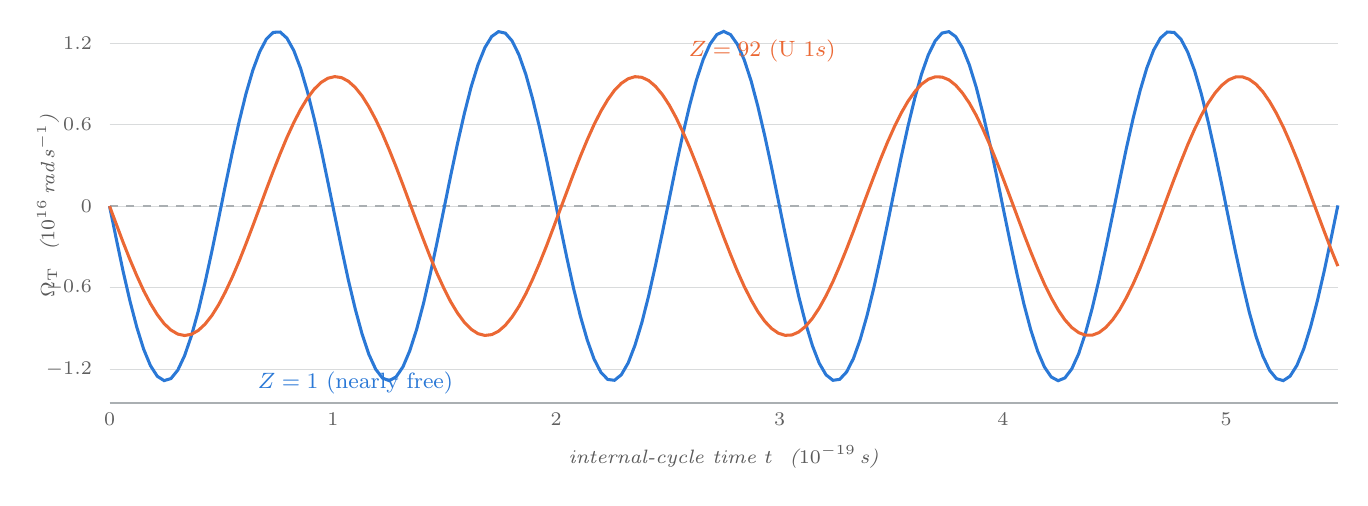
\begin{tikzpicture}[>=Stealth]
\definecolor{c1}{RGB}{42,120,214}
\definecolor{c2}{RGB}{235,104,52}
\definecolor{gr}{RGB}{170,175,178}
\draw[gr!45,line width=0.3pt] (0,0.431) -- (15.6,0.431);
\node[left,font=\scriptsize,gray!75!black] at (-0.10,0.431) {$-1.2$};
\draw[gr!45,line width=0.3pt] (0,1.466) -- (15.6,1.466);
\node[left,font=\scriptsize,gray!75!black] at (-0.10,1.466) {$-0.6$};
\draw[gr!45,line width=0.3pt] (0,2.500) -- (15.6,2.500);
\node[left,font=\scriptsize,gray!75!black] at (-0.10,2.500) {$0$};
\draw[gr!45,line width=0.3pt] (0,3.534) -- (15.6,3.534);
\node[left,font=\scriptsize,gray!75!black] at (-0.10,3.534) {$0.6$};
\draw[gr!45,line width=0.3pt] (0,4.569) -- (15.6,4.569);
\node[left,font=\scriptsize,gray!75!black] at (-0.10,4.569) {$1.2$};
\node[below,font=\scriptsize,gray!75!black] at (0.000,0.000) {$0$};
\node[below,font=\scriptsize,gray!75!black] at (2.836,0.000) {$1$};
\node[below,font=\scriptsize,gray!75!black] at (5.673,0.000) {$2$};
\node[below,font=\scriptsize,gray!75!black] at (8.509,0.000) {$3$};
\node[below,font=\scriptsize,gray!75!black] at (11.345,0.000) {$4$};
\node[below,font=\scriptsize,gray!75!black] at (14.182,0.000) {$5$};
\draw[gr,line width=0.5pt] (0,0.000) -- (15.6,0.000);
\draw[gr,line width=0.5pt,dashed] (0,2.500) -- (15.6,2.500);
\draw[c1,line width=1.1pt] plot coordinates {(0.000,2.500) (0.087,2.077) (0.173,1.669) (0.260,1.292) (0.347,0.959) (0.433,0.683) (0.520,0.473) (0.607,0.338) (0.693,0.283) (0.780,0.309) (0.867,0.416) (0.953,0.599) (1.040,0.852) (1.127,1.165) (1.213,1.528) (1.300,1.927) (1.387,2.346) (1.473,2.771) (1.560,3.186) (1.647,3.576) (1.733,3.927) (1.820,4.225) (1.907,4.459) (1.993,4.622) (2.080,4.706) (2.167,4.710) (2.253,4.632) (2.340,4.476) (2.427,4.247) (2.513,3.954) (2.600,3.608) (2.687,3.221) (2.773,2.807) (2.860,2.382) (2.947,1.962) (3.033,1.561) (3.120,1.195) (3.207,0.876) (3.293,0.618) (3.380,0.428) (3.467,0.315) (3.553,0.282) (3.640,0.331) (3.727,0.459) (3.813,0.662) (3.900,0.933) (3.987,1.261) (4.073,1.635) (4.160,2.041) (4.247,2.464) (4.333,2.887) (4.420,3.297) (4.507,3.678) (4.593,4.015) (4.680,4.296) (4.767,4.512) (4.853,4.653) (4.940,4.715) (5.027,4.696) (5.113,4.597) (5.200,4.420) (5.287,4.172) (5.373,3.863) (5.460,3.504) (5.547,3.109) (5.633,2.690) (5.720,2.265) (5.807,1.848) (5.893,1.456) (5.980,1.102) (6.067,0.799) (6.153,0.558) (6.240,0.389) (6.327,0.298) (6.413,0.287) (6.500,0.358) (6.587,0.508) (6.673,0.731) (6.760,1.018) (6.847,1.361) (6.933,1.745) (7.020,2.157) (7.107,2.581) (7.193,3.003) (7.280,3.406) (7.367,3.776) (7.453,4.098) (7.540,4.363) (7.627,4.558) (7.713,4.678) (7.800,4.718) (7.887,4.677) (7.973,4.555) (8.060,4.358) (8.147,4.093) (8.233,3.769) (8.320,3.398) (8.407,2.995) (8.493,2.573) (8.580,2.148) (8.667,1.737) (8.753,1.353) (8.840,1.012) (8.927,0.726) (9.013,0.504) (9.100,0.356) (9.187,0.287) (9.273,0.299) (9.360,0.392) (9.447,0.562) (9.533,0.804) (9.620,1.108) (9.707,1.463) (9.793,1.856) (9.880,2.273) (9.967,2.699) (10.053,3.117) (10.140,3.512) (10.227,3.870) (10.313,4.178) (10.400,4.424) (10.487,4.599) (10.573,4.697) (10.660,4.715) (10.747,4.651) (10.833,4.508) (10.920,4.291) (11.007,4.009) (11.093,3.670) (11.180,3.289) (11.267,2.879) (11.353,2.455) (11.440,2.033) (11.527,1.628) (11.613,1.254) (11.700,0.927) (11.787,0.657) (11.873,0.456) (11.960,0.329) (12.047,0.282) (12.133,0.317) (12.220,0.431) (12.307,0.622) (12.393,0.882) (12.480,1.202) (12.567,1.569) (12.653,1.970) (12.740,2.391) (12.827,2.816) (12.913,3.229) (13.000,3.615) (13.087,3.961) (13.173,4.252) (13.260,4.480) (13.347,4.634) (13.433,4.710) (13.520,4.705) (13.607,4.619) (13.693,4.455) (13.780,4.219) (13.867,3.920) (13.953,3.569) (14.040,3.178) (14.127,2.763) (14.213,2.338) (14.300,1.918) (14.387,1.521) (14.473,1.159) (14.560,0.846) (14.647,0.595) (14.733,0.413) (14.820,0.308) (14.907,0.283) (14.993,0.340) (15.080,0.477) (15.167,0.688) (15.253,0.965) (15.340,1.299) (15.427,1.677) (15.513,2.085) (15.600,2.508)};
\draw[c2,line width=1.1pt] plot coordinates {(0.000,2.500) (0.087,2.267) (0.173,2.038) (0.260,1.819) (0.347,1.614) (0.433,1.426) (0.520,1.261) (0.607,1.120) (0.693,1.007) (0.780,0.925) (0.867,0.874) (0.953,0.856) (1.040,0.871) (1.127,0.920) (1.213,1.000) (1.300,1.110) (1.387,1.249) (1.473,1.413) (1.560,1.599) (1.647,1.803) (1.733,2.021) (1.820,2.249) (1.907,2.482) (1.993,2.716) (2.080,2.945) (2.167,3.165) (2.253,3.371) (2.340,3.560) (2.427,3.728) (2.513,3.870) (2.600,3.985) (2.687,4.070) (2.773,4.123) (2.860,4.144) (2.947,4.131) (3.033,4.085) (3.120,4.007) (3.207,3.899) (3.293,3.762) (3.380,3.600) (3.467,3.416) (3.553,3.213) (3.640,2.996) (3.727,2.768) (3.813,2.536) (3.900,2.302) (3.987,2.073) (4.073,1.852) (4.160,1.644) (4.247,1.454) (4.333,1.284) (4.420,1.140) (4.507,1.022) (4.593,0.935) (4.680,0.879) (4.767,0.857) (4.853,0.867) (4.940,0.910) (5.027,0.986) (5.113,1.092) (5.200,1.226) (5.287,1.386) (5.373,1.569) (5.460,1.771) (5.547,1.987) (5.633,2.214) (5.720,2.447) (5.807,2.680) (5.893,2.910) (5.980,3.132) (6.067,3.341) (6.153,3.533) (6.240,3.704) (6.327,3.850) (6.413,3.970) (6.500,4.059) (6.587,4.117) (6.673,4.143) (6.760,4.135) (6.847,4.094) (6.933,4.021) (7.020,3.917) (7.107,3.785) (7.193,3.627) (7.280,3.445) (7.367,3.245) (7.453,3.030) (7.540,2.804) (7.627,2.571) (7.713,2.338) (7.800,2.107) (7.887,1.885) (7.973,1.675) (8.060,1.481) (8.147,1.309) (8.233,1.160) (8.320,1.038) (8.407,0.946) (8.493,0.886) (8.580,0.858) (8.667,0.863) (8.753,0.901) (8.840,0.972) (8.927,1.074) (9.013,1.204) (9.100,1.361) (9.187,1.540) (9.273,1.739) (9.360,1.954) (9.447,2.179) (9.533,2.411) (9.620,2.645) (9.707,2.875) (9.793,3.099) (9.880,3.310) (9.967,3.505) (10.053,3.679) (10.140,3.830) (10.227,3.953) (10.313,4.048) (10.400,4.111) (10.487,4.141) (10.573,4.138) (10.660,4.103) (10.747,4.034) (10.833,3.935) (10.920,3.807) (11.007,3.652) (11.093,3.474) (11.180,3.277) (11.267,3.063) (11.353,2.838) (11.440,2.607) (11.527,2.373) (11.613,2.142) (11.700,1.918) (11.787,1.706) (11.873,1.510) (11.960,1.334) (12.047,1.181) (12.133,1.055) (12.220,0.958) (12.307,0.893) (12.393,0.860) (12.480,0.860) (12.567,0.893) (12.653,0.959) (12.740,1.056) (12.827,1.182) (12.913,1.335) (13.000,1.511) (13.087,1.708) (13.173,1.920) (13.260,2.144) (13.347,2.375) (13.433,2.609) (13.520,2.841) (13.607,3.065) (13.693,3.279) (13.780,3.476) (13.867,3.654) (13.953,3.808) (14.040,3.936) (14.127,4.035) (14.213,4.103) (14.300,4.139) (14.387,4.141) (14.473,4.110) (14.560,4.047) (14.647,3.952) (14.733,3.828) (14.820,3.677) (14.907,3.503) (14.993,3.308) (15.080,3.097) (15.167,2.873) (15.253,2.642) (15.340,2.409) (15.427,2.177) (15.513,1.951) (15.600,1.737)};
\node[c1,font=\footnotesize,anchor=west] at (1.759,0.259) {$Z=1$ (nearly free)};
\node[c2,font=\footnotesize,anchor=west] at (7.233,4.466) {$Z=92$ (U $1s$)};
\node[below,font=\scriptsize\itshape,gray!70!black] at (7.800,-0.420) {internal-cycle time $t$ \ ($10^{-19}$\,s)};
\node[rotate=90,font=\scriptsize\itshape,gray!70!black] at (-0.78,2.500) {$\Omega_{\mathrm{T}}$ \ ($10^{16}$\,rad\,s$^{-1}$)};
\end{tikzpicture}
\caption{\textbf{The Thomas vortex over the internal cycle, free versus deeply bound}}
\label{fig:cycle}
\vspace{0.4em}
\begin{minipage}{0.95\textwidth}
\justifying\small
$\OmT(t)$ from Eq.~\eqref{eq:OmT} for a nearly free electron ($Z=1$, blue) and for the $1s$ electron of hydrogen-like uranium ($Z=92$, orange), computed with the canonical $\betaZB = 0.040472$ and the bound-state frequency of Eq.~\eqref{eq:omE}. Binding lowers the amplitude by $\gammaD = 0.7411$ and lengthens the period by $1/\gammaD = 1.3493$, so the two effects cancel in the cycle integral: the accumulated Thomas angle per cycle is $\vZB^{2}/c^{2} = 1.638\times10^{-3}$~rad for both curves, and indeed for every $Z$. The waveform is similar rather than distorted, which is the content of the statement that binding slows the internal clock without deforming the internal geometry.
\end{minipage}
\end{figure*}

\subsection{An Aside on a Recorded Open Item of Paper~\#50}
\label{subsec:p50}

Equation~\eqref{eq:invariant} allows a number to be attached to an open item Paper~\#50~\cite{hanamura50} recorded about itself. That paper requires an accumulated Thomas rotation of exactly $\pi$ per Zitterbewegung cycle, obtained from a discrete $n$-step construction with phase stagger $\delta b = \pi/n$, and notes that deriving this from the continuum Thomas rate formula $\OmT = (\gamma-1)(\vb{v}\times\vb{a})/v^{2}$ remains to be done. Paper~\#29~\cite{hanamura29} supplies the topological half of the statement --- a one-way traversal accumulates exactly $2\pi$ of spinorial phase through the line integral of the Thomas-precession connection --- so what is missing is specifically the bridge from that phase to the magnitude of the continuum rate. The continuum value from that formula is $2\pi\,a_e = 7.29\times10^{-3}$~rad; from the normalisation of Eq.~\eqref{eq:OmT} it is $1.64\times10^{-3}$~rad. The gap to $\pi$ is a factor $1/(2a_e) = 431.2$ in the first case and $1918$ in the second. We record the numbers without proposing a resolution, and note that entry C2 of the Corrections Log of Paper~\#66 bears on the same passage: the symbol $a$ carries at least three meanings across the corpus --- the monotonic internal phase of Paper~\#50, a kinematic convention in Papers~\#10 and~\#49, and the anomalous moment --- and the chirality computation of Paper~\#58 conflates the first two. Throughout the present paper $a$ denotes the anomalous magnetic moment and nothing else. For present purposes the relevant observation is that the discrepancy is a $Z$-independent normalisation and therefore does not propagate into either test of this paper.

% ========================================
\section{Test II: The Composition Side}
\label{sec:composition}
% ========================================

\subsection{$\betaZB$ Is Not a Universal Number}
\label{subsec:beta_species}

Test~I used $\betaZB$ only through the fact that it is a pure number, and never needed its value. The composition test needs its value, and needs it for more than one species.

Paper~\#61~\cite{hanamura61} applies the bridge equation directly to the proton, using the empirical anomalous moment $a_p = 1.7928$, and obtains a velocity-determining factor $\gv^{p} = 2.268$ and an internal velocity $\vZB^{p} \approx 0.898\,c$. Paper~\#62~\cite{hanamura62} discusses the sign convention for the neutron, whose moment is negative, and fixes the modulus form $\gamma = 1 + \lvert a\rvert$ precisely so that the equation can be applied to it. The bridge equation is therefore not restricted to the electron within the series; extending it across species is the series' own practice, not an extrapolation imposed from outside.

Table~\ref{tab:species} evaluates Eq.~\eqref{eq:bridge} for the four spin-$\tfrac12$ species whose anomalous moments are precisely known. The reproduced values agree with those quoted in Papers~\#51, \#61 and \#62. The pattern is stark. The two leptons agree with each other to $0.27\%$, because both anomalous moments are dominated by the same Schwinger term $\alpha/2\pi$. The two nucleons agree with each other to $0.85\%$. But the leptons and the nucleons differ by a factor of $22.2$, because the nucleon anomalous moments are of order unity rather than of order $10^{-3}$.

\begin{table*}[t!]
\centering
\caption{\textbf{The internal velocity $\betaZB$ across species from the bridge equation}}
\label{tab:species}
\renewcommand{\arraystretch}{1.4}
\begin{tabular}{p{2.2cm}p{2.8cm}p{2.0cm}p{2.0cm}p{2.3cm}p{3.2cm}}
\toprule
\textbf{Species} & \textbf{$\lvert a\rvert$} & \textbf{$\gv$} & \textbf{$\betaZB$} & \textbf{Ratio to $e$} & \textbf{Factor $1/\betaZB$ needed} \\
\midrule
electron
& 0.001159652
& 1.000820
& 0.040472
& 1.0000
& 24.708 \\
\addlinespace[0.3cm]
muon
& 0.001165921
& 1.000824
& 0.040581
& 1.0027
& 24.642 \\
\addlinespace[0.3cm]
proton
& 1.792847
& 2.267735
& 0.897522
& 22.176
& 1.114 \\
\addlinespace[0.3cm]
neutron
& 1.913043
& 2.352725
& 0.905175
& 22.366
& 1.105 \\
\addlinespace[0.2cm]
\bottomrule
\end{tabular}
\vspace{0.2cm}
\begin{minipage}{0.95\textwidth}
\justifying\footnotesize
Computed from Eq.~\eqref{eq:bridge} with the velocity-determining factor $\gv = 1 + \lvert a\rvert/\sqrt{2}$ of Papers~\#61 and~\#62. Inputs: $a_e$ from the Penning-trap measurement of the electron magnetic moment~\cite{fan2023}; $a_\mu$ from the Fermilab Muon $g-2$ final result~\cite{muong2_2025}; $a_p = \mu_p/\mu_N - 1$ and $\lvert a_n\rvert = \lvert\mu_n\rvert/\mu_N$ from CODATA~\cite{codata2022}. The reproduced proton value $0.8975\,c$ agrees with the $0.898\,c$ quoted in Paper~\#61 and the electron value $0.04047\,c$ with Papers~\#51 and~\#62. The last column is the factor by which Eq.~\eqref{eq:F52} falls short of the Newtonian $F = mg$ for that species: it is not a constant.
\end{minipage}
\end{table*}

\subsection{The Consequence for Bulk Matter}
\label{subsec:bulk}

Reading Eq.~\eqref{eq:F52} literally and species by species, a body made of $N_e$ electrons and $N_N$ nucleons experiences a total gravitational force proportional to $\sum_s m_s \betaZB^{s}$ rather than to $\sum_s m_s$. Normalising to the nucleon value, the ratio of gravitational to inertial mass becomes
\begin{equation}
\frac{m_g}{m_i} \;=\; x_e\,\frac{\betaZB^{e}}{\betaZB^{p}} + (1-x_e),
\label{eq:mgmi}
\end{equation}
where $x_e$ is the electron mass fraction of the material. Since $\betaZB^{e}/\betaZB^{p} = 0.0451$, electrons contribute only $4.5\%$ of the gravitational pull that their mass would suggest, and a material with more electrons per unit mass falls more slowly.

The electron mass fraction is $2.521\times10^{-4}$ for titanium and $2.193\times10^{-4}$ for platinum, the difference arising because platinum has a larger neutron excess and therefore fewer electrons per unit mass. Equation~\eqref{eq:mgmi} then predicts
\begin{equation}
\eta(\mathrm{Ti},\mathrm{Pt}) \;=\; 3.13\times10^{-5},
\label{eq:eta_pred}
\end{equation}
against the MICROSCOPE bound of $2.7\times10^{-15}$~\cite{microscope2022}. The prediction exceeds the bound by a factor of $1.2\times10^{10}$. Figure~\ref{fig:eta} places this and three other material pairs on a logarithmic axis alongside the measured bound.

\subsection{The Nuclear-Binding Lever}
\label{subsec:nuclear_lever}

A second and independent lever constrains a different family of readings. Suppose the gravitational charge were not linear in energy --- for instance if one identified it with the rate of fragment emission times the energy per fragment, which scales as $\omZB^{2} \propto E^{2}$. Then the mass defect would be doubled at leading order, and since nuclear binding accounts for roughly $0.9\%$ of the mass of ordinary matter and varies between nuclides, the doubling would show up directly in $\eta$.

The nuclear binding fraction is $9.375\times10^{-3}$ for $^{48}$Ti and $8.511\times10^{-3}$ for $^{195}$Pt, so a charge quadratic in energy predicts $\eta(\mathrm{Ti},\mathrm{Pt}) = 8.64\times10^{-4}$, exceeding the bound by $3.2\times10^{11}$. For the pair $^{9}$Be and $^{238}$U the prediction is $1.20\times10^{-3}$. The same reading is also excluded, far less strongly but far more directly, by the mass of the hydrogen atom: doubling the $13.6$~eV defect would shift $m(^{1}\mathrm{H})$ by $1.46\times10^{-8}$~u against an uncertainty of $9\times10^{-11}$~u~\cite{ame2020}, a discrepancy of $162\sigma$.

Figure~\ref{fig:fork} shows the bound-state form of the same statement: the gravitating mass of a $1s$ electron as a function of $Z$ for charges scaling as $E$, $E^{2}$ and $E^{3}$. Only the first is consistent with the equivalence principle; at $Z = 92$ the second is wrong by $98.0$~keV and the third by $170.7$~keV.

\begin{figure*}[t!]
\centering
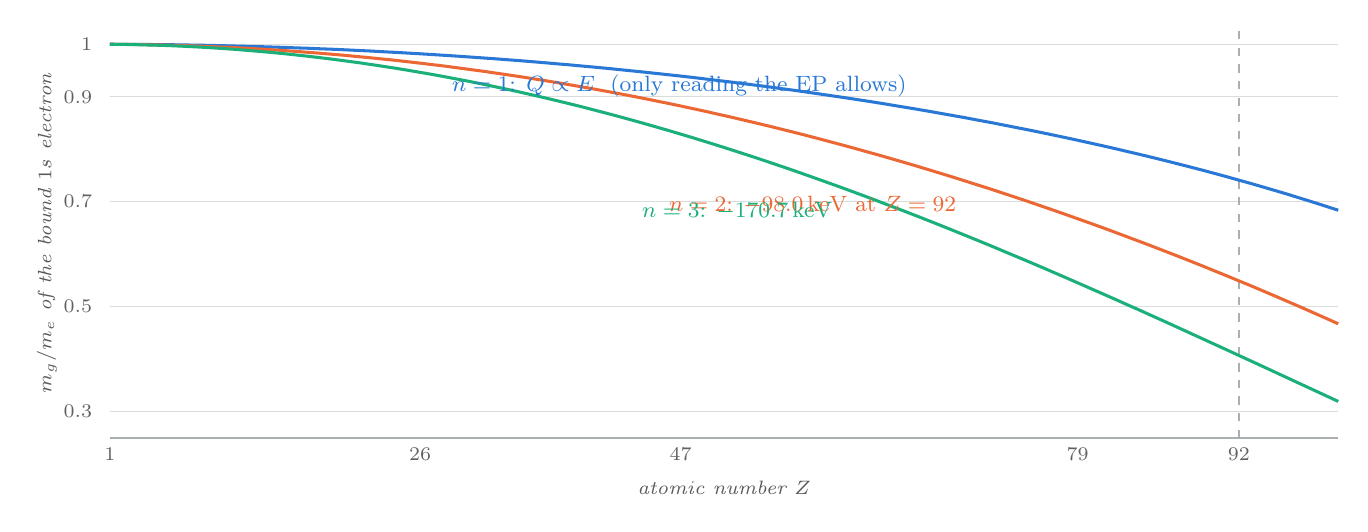
\begin{tikzpicture}[>=Stealth]
\definecolor{c1}{RGB}{42,120,214}
\definecolor{c2}{RGB}{235,104,52}
\definecolor{c3}{RGB}{27,175,122}
\definecolor{gr}{RGB}{170,175,178}
\draw[gr!45,line width=0.3pt] (0,0.333) -- (15.6,0.333);
\node[left,font=\scriptsize,gray!75!black] at (-0.10,0.333) {$0.3$};
\draw[gr!45,line width=0.3pt] (0,1.667) -- (15.6,1.667);
\node[left,font=\scriptsize,gray!75!black] at (-0.10,1.667) {$0.5$};
\draw[gr!45,line width=0.3pt] (0,3.000) -- (15.6,3.000);
\node[left,font=\scriptsize,gray!75!black] at (-0.10,3.000) {$0.7$};
\draw[gr!45,line width=0.3pt] (0,4.333) -- (15.6,4.333);
\node[left,font=\scriptsize,gray!75!black] at (-0.10,4.333) {$0.9$};
\draw[gr!45,line width=0.3pt] (0,5.000) -- (15.6,5.000);
\node[left,font=\scriptsize,gray!75!black] at (-0.10,5.000) {$1$};
\node[below,font=\scriptsize,gray!75!black] at (0.000,0.000) {$1$};
\node[below,font=\scriptsize,gray!75!black] at (3.939,0.000) {$26$};
\node[below,font=\scriptsize,gray!75!black] at (7.248,0.000) {$47$};
\node[below,font=\scriptsize,gray!75!black] at (12.291,0.000) {$79$};
\node[below,font=\scriptsize,gray!75!black] at (14.339,0.000) {$92$};
\draw[gr,line width=0.5pt] (0,0.000) -- (15.6,0.000);
\draw[gr,line width=0.6pt,dashed] (14.339,0.000) -- (14.339,5.200);
\draw[c1,line width=1.1pt] plot coordinates {(0.000,5.000) (0.158,4.999) (0.315,4.998) (0.473,4.997) (0.630,4.996) (0.788,4.994) (0.945,4.991) (1.103,4.989) (1.261,4.986) (1.418,4.982) (1.576,4.978) (1.733,4.974) (1.891,4.970) (2.048,4.965) (2.206,4.960) (2.364,4.954) (2.521,4.949) (2.679,4.942) (2.836,4.936) (2.994,4.929) (3.152,4.921) (3.309,4.914) (3.467,4.905) (3.624,4.897) (3.782,4.888) (3.939,4.879) (4.097,4.869) (4.255,4.859) (4.412,4.849) (4.570,4.838) (4.727,4.827) (4.885,4.816) (5.042,4.804) (5.200,4.792) (5.358,4.779) (5.515,4.766) (5.673,4.752) (5.830,4.739) (5.988,4.724) (6.145,4.710) (6.303,4.695) (6.461,4.679) (6.618,4.663) (6.776,4.647) (6.933,4.630) (7.091,4.613) (7.248,4.596) (7.406,4.578) (7.564,4.559) (7.721,4.540) (7.879,4.521) (8.036,4.501) (8.194,4.481) (8.352,4.461) (8.509,4.439) (8.667,4.418) (8.824,4.396) (8.982,4.373) (9.139,4.350) (9.297,4.327) (9.455,4.303) (9.612,4.279) (9.770,4.254) (9.927,4.228) (10.085,4.202) (10.242,4.176) (10.400,4.149) (10.558,4.121) (10.715,4.093) (10.873,4.065) (11.030,4.035) (11.188,4.006) (11.345,3.975) (11.503,3.944) (11.661,3.913) (11.818,3.881) (11.976,3.848) (12.133,3.815) (12.291,3.781) (12.448,3.746) (12.606,3.711) (12.764,3.675) (12.921,3.638) (13.079,3.601) (13.236,3.563) (13.394,3.524) (13.552,3.484) (13.709,3.444) (13.867,3.403) (14.024,3.361) (14.182,3.318) (14.339,3.274) (14.497,3.230) (14.655,3.184) (14.812,3.138) (14.970,3.091) (15.127,3.042) (15.285,2.993) (15.442,2.943) (15.600,2.892)};
\draw[c2,line width=1.1pt] plot coordinates {(0.000,5.000) (0.158,4.999) (0.315,4.997) (0.473,4.994) (0.630,4.991) (0.788,4.987) (0.945,4.983) (1.103,4.977) (1.261,4.971) (1.418,4.964) (1.576,4.957) (1.733,4.949) (1.891,4.940) (2.048,4.930) (2.206,4.920) (2.364,4.909) (2.521,4.897) (2.679,4.885) (2.836,4.872) (2.994,4.858) (3.152,4.843) (3.309,4.828) (3.467,4.812) (3.624,4.796) (3.782,4.778) (3.939,4.760) (4.097,4.741) (4.255,4.722) (4.412,4.701) (4.570,4.680) (4.727,4.659) (4.885,4.636) (5.042,4.613) (5.200,4.590) (5.358,4.565) (5.515,4.540) (5.673,4.514) (5.830,4.487) (5.988,4.460) (6.145,4.432) (6.303,4.403) (6.461,4.374) (6.618,4.344) (6.776,4.313) (6.933,4.281) (7.091,4.249) (7.248,4.216) (7.406,4.182) (7.564,4.148) (7.721,4.112) (7.879,4.077) (8.036,4.040) (8.194,4.003) (8.352,3.965) (8.509,3.926) (8.667,3.887) (8.824,3.847) (8.982,3.806) (9.139,3.764) (9.297,3.722) (9.455,3.679) (9.612,3.635) (9.770,3.591) (9.927,3.546) (10.085,3.500) (10.242,3.454) (10.400,3.406) (10.558,3.358) (10.715,3.310) (10.873,3.260) (11.030,3.210) (11.188,3.160) (11.345,3.108) (11.503,3.056) (11.661,3.003) (11.818,2.949) (11.976,2.895) (12.133,2.840) (12.291,2.784) (12.448,2.728) (12.606,2.671) (12.764,2.613) (12.921,2.554) (13.079,2.495) (13.236,2.435) (13.394,2.374) (13.552,2.313) (13.709,2.251) (13.867,2.188) (14.024,2.124) (14.182,2.060) (14.339,1.995) (14.497,1.930) (14.655,1.863) (14.812,1.796) (14.970,1.728) (15.127,1.660) (15.285,1.590) (15.442,1.521) (15.600,1.450)};
\draw[c3,line width=1.1pt] plot coordinates {(0.000,4.999) (0.158,4.998) (0.315,4.995) (0.473,4.991) (0.630,4.987) (0.788,4.981) (0.945,4.974) (1.103,4.966) (1.261,4.957) (1.418,4.947) (1.576,4.936) (1.733,4.923) (1.891,4.910) (2.048,4.896) (2.206,4.881) (2.364,4.864) (2.521,4.847) (2.679,4.828) (2.836,4.809) (2.994,4.788) (3.152,4.767) (3.309,4.744) (3.467,4.720) (3.624,4.696) (3.782,4.670) (3.939,4.643) (4.097,4.616) (4.255,4.587) (4.412,4.557) (4.570,4.527) (4.727,4.495) (4.885,4.462) (5.042,4.429) (5.200,4.394) (5.358,4.358) (5.515,4.322) (5.673,4.284) (5.830,4.246) (5.988,4.207) (6.145,4.166) (6.303,4.125) (6.461,4.083) (6.618,4.040) (6.776,3.996) (6.933,3.951) (7.091,3.906) (7.248,3.859) (7.406,3.812) (7.564,3.763) (7.721,3.714) (7.879,3.664) (8.036,3.613) (8.194,3.562) (8.352,3.509) (8.509,3.456) (8.667,3.402) (8.824,3.347) (8.982,3.291) (9.139,3.235) (9.297,3.178) (9.455,3.120) (9.612,3.062) (9.770,3.002) (9.927,2.942) (10.085,2.882) (10.242,2.821) (10.400,2.759) (10.558,2.696) (10.715,2.633) (10.873,2.569) (11.030,2.505) (11.188,2.440) (11.345,2.374) (11.503,2.308) (11.661,2.242) (11.818,2.175) (11.976,2.107) (12.133,2.039) (12.291,1.970) (12.448,1.901) (12.606,1.832) (12.764,1.762) (12.921,1.692) (13.079,1.622) (13.236,1.551) (13.394,1.480) (13.552,1.408) (13.709,1.336) (13.867,1.264) (14.024,1.192) (14.182,1.120) (14.339,1.047) (14.497,0.975) (14.655,0.902) (14.812,0.829) (14.970,0.756) (15.127,0.683) (15.285,0.610) (15.442,0.537) (15.600,0.464)};
\node[c1,font=\footnotesize,anchor=east] at (10.242,4.476) {$n=1$: $Q\propto E$ \ (only reading the EP allows)};
\node[c2,font=\footnotesize,anchor=east] at (10.873,2.960) {$n=2$: $-98.0$\,keV at $Z=92$};
\node[c3,font=\footnotesize,anchor=east] at (9.297,2.878) {$n=3$: $-170.7$\,keV};
\node[below,font=\scriptsize\itshape,gray!70!black] at (7.800,-0.420) {atomic number $Z$};
\node[rotate=90,font=\scriptsize\itshape,gray!70!black] at (-0.80,2.600) {$m_g/m_e$ of the bound $1s$ electron};
\end{tikzpicture}
\caption{\textbf{Gravitating mass of a bound $1s$ electron for three readings of the charge}}
\label{fig:fork}
\vspace{0.4em}
\begin{minipage}{0.95\textwidth}
\justifying\small
The equivalence principle fixes the gravitating mass of a $1s$ electron at $\gammaD\,m_e$, the $n=1$ curve. A gravitational charge scaling as $E^{2}$ --- the reading in which the charge is identified with the emission power rather than the energy content --- gives the $n=2$ curve, which at low $Z$ doubles the binding-energy mass defect exactly and at $Z=92$ is short by $98.0$~keV. A charge scaling as $E^{3}$, which is what one obtains from Eq.~\eqref{eq:OmT_E} if $\vZB$ is allowed to scale with the binding, is short by $170.7$~keV. The dashed vertical line marks hydrogen-like uranium, where the separation between the readings is largest and least ambiguous.
\end{minipage}
\end{figure*}

\begin{figure*}[t!]
\centering
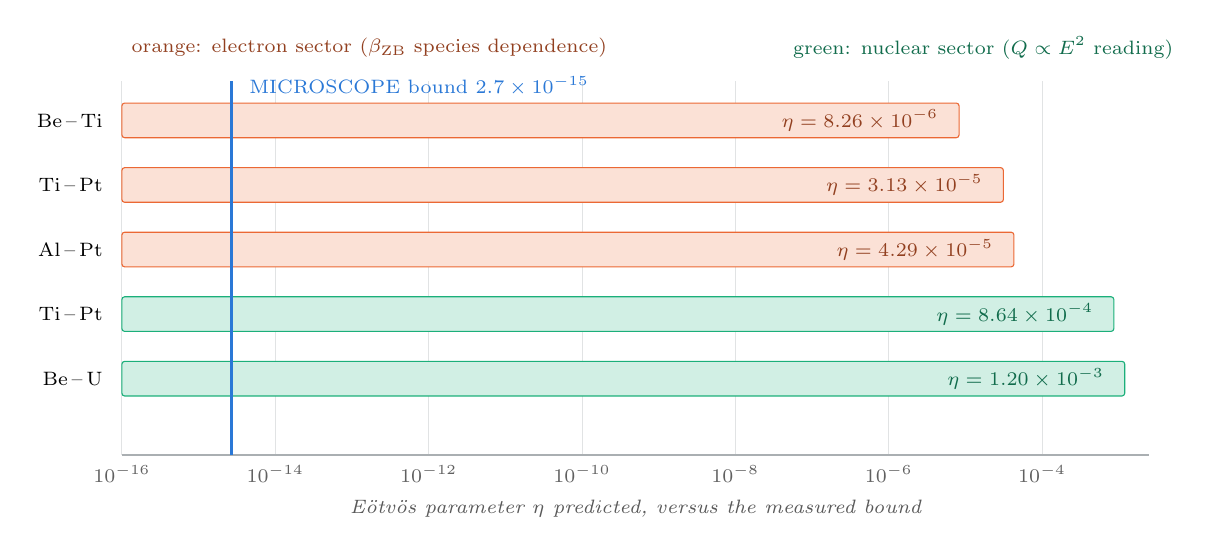
\begin{tikzpicture}[>=Stealth]
\definecolor{c2}{RGB}{235,104,52}
\definecolor{c3}{RGB}{27,175,122}
\definecolor{c1}{RGB}{42,120,214}
\definecolor{gr}{RGB}{170,175,178}
\draw[gr!35,line width=0.3pt] (2.550,0.15) -- (2.550,4.900);
\node[below,font=\scriptsize,gray!75!black] at (2.550,0.15) {$10^{-16}$};
\draw[gr!35,line width=0.3pt] (4.498,0.15) -- (4.498,4.900);
\node[below,font=\scriptsize,gray!75!black] at (4.498,0.15) {$10^{-14}$};
\draw[gr!35,line width=0.3pt] (6.446,0.15) -- (6.446,4.900);
\node[below,font=\scriptsize,gray!75!black] at (6.446,0.15) {$10^{-12}$};
\draw[gr!35,line width=0.3pt] (8.393,0.15) -- (8.393,4.900);
\node[below,font=\scriptsize,gray!75!black] at (8.393,0.15) {$10^{-10}$};
\draw[gr!35,line width=0.3pt] (10.341,0.15) -- (10.341,4.900);
\node[below,font=\scriptsize,gray!75!black] at (10.341,0.15) {$10^{-8}$};
\draw[gr!35,line width=0.3pt] (12.289,0.15) -- (12.289,4.900);
\node[below,font=\scriptsize,gray!75!black] at (12.289,0.15) {$10^{-6}$};
\draw[gr!35,line width=0.3pt] (14.237,0.15) -- (14.237,4.900);
\node[below,font=\scriptsize,gray!75!black] at (14.237,0.15) {$10^{-4}$};
\draw[gr,line width=0.5pt] (2.550,0.15) -- (15.600,0.15);
\draw[c2,line width=0.4pt,fill=c2!20,rounded corners=1pt] (2.550,4.180) rectangle (13.182,4.620);
\node[left,font=\scriptsize] at (2.430,4.400) {Be\,--\,Ti};
\node[left,font=\scriptsize,c2!62!black] at (13.042,4.400) {$\eta=8.26\times 10^{-6}$};
\draw[c2,line width=0.4pt,fill=c2!20,rounded corners=1pt] (2.550,3.360) rectangle (13.745,3.800);
\node[left,font=\scriptsize] at (2.430,3.580) {Ti\,--\,Pt};
\node[left,font=\scriptsize,c2!62!black] at (13.605,3.580) {$\eta=3.13\times 10^{-5}$};
\draw[c2,line width=0.4pt,fill=c2!20,rounded corners=1pt] (2.550,2.540) rectangle (13.879,2.980);
\node[left,font=\scriptsize] at (2.430,2.760) {Al\,--\,Pt};
\node[left,font=\scriptsize,c2!62!black] at (13.739,2.760) {$\eta=4.29\times 10^{-5}$};
\draw[c3,line width=0.4pt,fill=c3!20,rounded corners=1pt] (2.550,1.720) rectangle (15.148,2.160);
\node[left,font=\scriptsize] at (2.430,1.940) {Ti\,--\,Pt};
\node[left,font=\scriptsize,c3!62!black] at (15.008,1.940) {$\eta=8.64\times 10^{-4}$};
\draw[c3,line width=0.4pt,fill=c3!20,rounded corners=1pt] (2.550,0.900) rectangle (15.286,1.340);
\node[left,font=\scriptsize] at (2.430,1.120) {Be\,--\,U};
\node[left,font=\scriptsize,c3!62!black] at (15.146,1.120) {$\eta=1.20\times 10^{-3}$};
\draw[c1,line width=1.1pt] (3.944,0.15) -- (3.944,4.900);
\node[c1,font=\scriptsize,anchor=west] at (4.044,4.840) {MICROSCOPE bound $2.7\times10^{-15}$};
\node[c2!62!black,font=\scriptsize,anchor=west] at (2.650,3.890) {};
\node[below,font=\scriptsize\itshape,gray!70!black] at (9.075,-0.30) {E\"otv\"os parameter $\eta$ predicted, versus the measured bound};
\node[c2!62!black,font=\scriptsize,anchor=west] at (2.550,5.320) {orange: electron sector ($\beta_{\mathrm{ZB}}$ species dependence)};
\node[c3!62!black,font=\scriptsize,anchor=west] at (10.950,5.320) {green: nuclear sector ($Q\propto E^2$ reading)};
\end{tikzpicture}
\caption{\textbf{Predicted E\"otv\"os parameters against the measured bound}}
\label{fig:eta}
\vspace{0.4em}
\begin{minipage}{0.95\textwidth}
\justifying\small
Orange bars: composition dependence induced by the species dependence of $\betaZB$ through Eq.~\eqref{eq:mgmi}, for four material pairs. Green bars: composition dependence induced by a gravitational charge quadratic in energy, acting through the nuclear binding fraction. The blue line is the MICROSCOPE sensitivity $2.7\times10^{-15}$~\cite{microscope2022}. The horizontal axis is logarithmic and spans thirteen decades; the smallest predicted effect exceeds the measured bound by more than nine orders of magnitude. The nuclear lever is the stronger of the two because nuclear binding is a larger and more variable fraction of mass than the electron content.
\end{minipage}
\end{figure*}

\subsection{Candidate Readings and What Each Requires}
\label{subsec:candidates}

Table~\ref{tab:verdict} collects the readings of ``gravitational charge'' that the series makes available and the verdict on each. The pattern is simple enough to state in words. A charge linear in the total energy passes every test. A charge non-linear in energy is excluded by the nuclear lever. And a charge containing $\vZB$ at any power is excluded by the species lever, because $\vZB$ is not universal.

\begin{table*}[t!]
\centering
\caption{\textbf{Readings of the gravitational charge and the constraint on each}}
\label{tab:verdict}
\renewcommand{\arraystretch}{1.4}
\setlength{\tabcolsep}{8pt}
\begin{tabular}{p{3.2cm}p{2.9cm}p{1.7cm}p{3.4cm}p{3.1cm}}
\toprule
\textbf{Reading} & \textbf{Source} & \textbf{Scaling} & \textbf{Strongest constraint} & \textbf{Verdict} \\
\midrule
Total energy $E$ alone
& equivalence principle
& $E^{1}$, no $\vZB$
& ---
& survives \\
\addlinespace[0.3cm]
Fragment energy $\hbar\omZB$
& \#49
& $E^{1}$, $\vZB^{1}$
& species lever, $1.2\times10^{10}$
& excluded as written \\
\addlinespace[0.3cm]
Thomas vortex $\OmT$
& \#58, Eq.~\eqref{eq:OmT}
& $E^{1}$, $\vZB^{3}$
& species lever, $1.2\times10^{10}$
& excluded as written \\
\addlinespace[0.3cm]
Force law $mg\,\betaZB$
& \#52, Eq.~\eqref{eq:F52}
& $E^{1}$, $\vZB^{1}$
& species lever, $1.2\times10^{10}$
& must cancel $\betaZB$ \\
\addlinespace[0.3cm]
Emission power
& emission picture
& $E^{2}$
& nuclear lever, $3.2\times10^{11}$
& excluded \\
\addlinespace[0.3cm]
$\OmT$ with $\vZB \propto E$
& \#63, horizon
& $E^{3}$
& bound state, $170.7$~keV
& excluded \\
\addlinespace[0.2cm]
\bottomrule
\end{tabular}
\vspace{0.2cm}
\begin{minipage}{0.95\textwidth}
\justifying\footnotesize
``Excluded as written'' means that the quantity cannot be the coupling strength in the form stated; it does not mean that the quantity plays no role, and Section~\ref{sec:survives} argues that $\OmT$ retains a different and well-defined role. Exclusion factors are the ratio of the predicted E\"otv\"os parameter for the Ti--Pt pair to the MICROSCOPE sensitivity $2.7\times10^{-15}$.
\end{minipage}
\end{table*}

% ========================================
\section{What Survives, and What It Asks of the Completing Mechanism}
\label{sec:survives}
% ========================================

\subsection{A Division of Labour}
\label{subsec:division}

The two tests together point to a single reorganisation, and it is one the series is already close to making. Paper~\#58's argument for $\OmT$ is that its $\pi$-periodicity supplies the rank-2, spin-2 \emph{polarisation} structure of the mediator --- that is, it is an argument about what kind of field gravity is, not about how strongly it couples. Nothing in that argument requires $\OmT$ also to set the coupling strength. The results above say that it must not:
\begin{align}
\underbrace{\OmT}_{\text{$\pi$-periodic, rank-2}}
&\;\longrightarrow\;
\underbrace{\text{spin of the mediator}}_{\text{polarisation structure}}
\notag\\
\underbrace{E}_{\text{total energy}}
&\;\longrightarrow\;
\underbrace{\text{strength of the coupling}}_{\text{gravitational charge}} .
\label{eq:division}
\end{align}
Read this way, the composition test does not remove anything the series has established. It removes an identification the series had left implicit, and replaces it with a sharper one.

\subsection{The Constraint on Paper~\#52's Open Task}
\label{subsec:constraint}

Paper~\#52 recorded the recovery of $F = mg$ from $F = mg\,\betaZB$ as an open task, and it is natural to read such a task as the search for a missing factor of about $25$. Table~\ref{tab:species} shows that this reading is not available. The factor required is $24.71$ for an electron, $24.64$ for a muon, $1.114$ for a proton and $1.105$ for a neutron. A mechanism that supplies a universal constant cannot do the job; a mechanism that supplies a factor $1/\betaZB$ can, and is the only kind that can. Stated as a requirement:

\paragraph{Completion requirement.} \emph{Any mechanism completing the derivation of Paper~\#52 must supply a factor exactly equal to $1/\betaZB$ for each species, so that $\vZB$ cancels from the gravitational force identically. Equivalently: the number of internal cycles per unit time and the momentum transferred per cycle must combine so that the internal speed does not survive in the product.}

This is a constructive statement, and it is testable inside the model rather than only against experiment. It says where to look: at whatever governs the probability that a given internal cycle actually results in an exchange. If that probability is itself proportional to $1/\betaZB$ --- if slower internal motion is compensated by more efficient exchange --- then the cancellation is structural in the same sense that Paper~\#52's $\lambdaC$ cancellation is structural, and the same style of argument would complete it. The suppression factor $\epsilon_2\epsilon_3 \sim 10^{-5}$ introduced in Papers~\#34 and~\#49 is the natural place for such a dependence to live, and we note without developing it that this is the first quantitative demand the series has placed on that factor.

\subsection{A Second, Weaker Handle}
\label{subsec:muon}

If the composition problem were resolved by some means other than cancelling $\betaZB$, a residual prediction would remain that is far smaller and currently unconstrained. Because $a_\mu$ and $a_e$ differ by $0.54\%$, the readings that retain $\betaZB$ predict that a muon and an electron gravitate differently per unit mass by $0.27\%$. No experiment approaches this sensitivity for muons, so it is not presently a test; we record it because it is the one place where the species dependence appears within a single family and is therefore free of the composite-structure caveat of Section~\ref{subsec:composite}.

% ========================================
\section{An Incompatibility Between Papers~\#62 and~\#63, and Its Resolution}
\label{sec:tension}
% ========================================

\subsection{The Two Statements}
\label{subsec:two_statements}

Test~I turned on $\vZB$ being a pure number, so it is worth asking whether the series says anywhere that it is not. It does.

Paper~\#62~\cite{hanamura62} argues that the anomalous moment is a single frame-independent invariant with an internal geometric representation, and is explicit about its field-independence. Since $\betaZB$ is a function of $a$ alone through Eq.~\eqref{eq:bridge}, this makes $\betaZB$ a constant of nature.

Paper~\#63~\cite{hanamura63} makes a structural prediction about strong gravitational fields. Following the redshift of internal clocks established in Paper~\#22~\cite{hanamura22}, it argues that as the horizon is approached the internal frequency and with it the transverse speed $\vZB$ are driven to zero, so that $\OmT \propto \vZB^{2}$ vanishes, fragment ejection ceases, and the gravitational coupling freezes out rather than diverging as the curvature of general relativity does.

The two cannot both be local statements. If $\betaZB$ is fixed by a field-independent $a$, it cannot go to zero anywhere. If it goes to zero locally, then $a$ depends on the gravitational potential.

\subsection{The Two Readings}
\label{subsec:ways_out}

\paragraph{Reading A: $\vZB$ is a local invariant.} Test~I then stands as derived, and Paper~\#63's freezing is a statement about quantities measured by a distant observer rather than about local physics. This is internally consistent, but it costs the prediction its interest: general relativity already predicts that a distant observer sees internal processes freeze near the horizon, so the freezing is no longer a point of divergence from general relativity.

\paragraph{Reading B: $\vZB$ decreases locally.} Then $a$ carries a dependence on the gravitational potential $\Phi$. If $\vZB \propto \sqrt{1 + 2\Phi/c^{2}}$, as the redshift argument suggests, then from $\betaZB^{2} \approx \sqrt{2}\,\lvert a\rvert$ one obtains $a \propto (1 + 2\Phi/c^{2})$ to leading order, that is
\begin{equation}
k_{a} \;\equiv\; \frac{c^{2}}{a}\,\dv{a}{\Phi} \;=\; 2 .
\label{eq:ka}
\end{equation}
This is a violation of local position invariance with a coefficient of order unity, and local position invariance is measured.

\subsection{Reading B Is Excluded by Existing Clock Comparisons}
\label{subsec:LPI}

The coefficient defined in Eq.~\eqref{eq:ka} is exactly the quantity that clock-comparison experiments bound for the fundamental constants, using the annual modulation of the solar gravitational potential at the Earth as the lever. Ferrell \textit{et al.}~\cite{ferrell2007} monitored nearly degenerate opposite-parity levels of atomic dysprosium over eight months and obtained $k_\alpha = (-8.7 \pm 6.6)\times10^{-6}$ for the fine-structure constant. Lange \textit{et al.}~\cite{lange2021}, comparing the electric-quadrupole and electric-octupole clock transitions of $^{171}$Yb$^{+}$ against caesium fountains over several years, improved this to
\begin{equation}
k_\alpha \;=\; \frac{c^{2}}{\alpha}\dv{\alpha}{\Phi} \;=\; 14(11)\times10^{-9},
\label{eq:kalpha}
\end{equation}
together with $k_\mu = 7(45)\times10^{-8}$ for the proton-to-electron mass ratio.

In standard quantum electrodynamics the electron anomaly is a function of the fine-structure constant, $a_e = \alpha/2\pi - 0.328\,(\alpha/\pi)^{2} + \dots$, so at leading order $k_{a} = k_\alpha$. Comparing Eq.~\eqref{eq:ka} with Eq.~\eqref{eq:kalpha}, Reading~B requires a coefficient of $2$ where measurement bounds it below $2.5\times10^{-8}$. \emph{Reading~B is excluded by eight orders of magnitude}, and was already excluded by five orders of magnitude by the dysprosium measurement of 2007.

One loophole remains, and it should be stated rather than passed over. The bound of Eq.~\eqref{eq:kalpha} constrains $\alpha$, and the series does not derive $a_e$ from $\alpha$ --- Paper~\#10 takes the measured anomaly as empirical input. One could therefore hold that $a_e$ varies with $\Phi$ while $\alpha$ does not, in which case Eq.~\eqref{eq:kalpha} does not apply directly. The cost of that position is high. It requires the agreement between the measured $a_e$ and the QED series in $\alpha$, which holds to ten significant figures at our own gravitational potential, to be a coincidence that dissolves elsewhere. We do not think this can be maintained, but we note the experiment that would test it, since it is the one remaining discriminant. Because $a_e$ is determined in a Penning trap as the ratio $\nu_a/\nu_c$ of the anomaly to the cyclotron frequency, a common redshift of the apparatus cancels exactly in the ratio, so any residual annual dependence would be a real violation and not a clock artefact. With $\Delta\Phi/c^{2} = 2e\,GM_\odot/(a_\oplus c^{2}) = 3.299\times10^{-10}$ over the year, Reading~B predicts an annual modulation of the measured moment of $\Delta(g/2) = a_e\,k_a\,\Delta\Phi/c^{2} = 7.65\times10^{-13}$, against the single-measurement uncertainty $1.3\times10^{-13}$ of Ref.~\cite{fan2023} --- a ratio of $5.9$. That comparison is idealised: extracting an annual modulation would require a campaign with data distributed across the year and control of systematics correlated with season. We record it as the residual test of a narrow hypothesis, not as a headline proposal.

\subsection{Consequence for the Series}
\label{subsec:tension_consequence}

Reading~A is therefore forced. Three things follow.

First, Test~I stands without qualification: $\vZB$ is a local invariant, so the reduction $\OmT \propto E$ of Section~\ref{subsec:OmT_reduce} is not threatened from this direction.

Second, the horizon-freezing prediction of Paper~\#63 must be read as a statement about quantities inferred by a distant observer. So read, it is not in conflict with general relativity and not a test of the model against it. Paper~\#63 flagged the prediction as structural rather than quantitative and as an ``in-principle-testable point of divergence''; the present analysis removes the divergence while leaving the structural statement intact. The series should not count it as an observational signature.

Third, and more generally, the episode illustrates a hazard that the framework will meet repeatedly. Because $\betaZB$ is anchored to a measured constant, any proposal that makes the internal kinematics respond to the environment converts immediately into a claim that a measured constant varies --- and measured constants are bounded very tightly indeed. The same arithmetic that makes the model pass Test~I makes it unable to purchase environmental responses cheaply.

% ========================================
\section{Diagnosis: One Mismatch in Four Disguises, and Where the Formalisation Should Restart}
\label{sec:diagnosis}
% ========================================

\subsection{Four Symptoms, One Mismatch}
\label{subsec:four_symptoms}

The results of Sections~\ref{sec:composition} and~\ref{sec:tension} look like four separate difficulties. They are not. Table~\ref{tab:diagnosis} collects them, and the common structure is visible once they are set side by side: in every case an \emph{internal kinematic} quantity has been asked to carry the \emph{gravitational charge}.

The mismatch is then immediate. Internal kinematic quantities are anchored, through the bridge equation, to the measured anomalous moment, and are therefore species-specific: $\betaZB$ is $0.0405$ for a lepton and $0.898$ for a nucleon. The gravitational charge, by contrast, must be the total energy and nothing else, to one part in $10^{15}$. A quantity fixed by $a$ cannot be a quantity fixed by $E$, and every construction that routes the charge through the internal kinematics inherits the contradiction in one form or another.

There is an irony worth stating plainly, because it is the sharpest thing this paper has to say about the framework. \emph{The same property that makes the model pass Test~I makes it fail Test~II.} Test~I succeeds because $\betaZB$ is a pure number, so binding cannot change it and the charge tracks $E$ alone. Test~II fails because it is a \emph{different} pure number for each species, so composition does change it. One property, two consequences, in opposite directions. This is not a defect that can be repaired by adjusting the value of $\betaZB$; no value works, because the problem is that the charge depends on it at all.

\begin{table*}[t!]
\centering
\caption{\textbf{Four symptoms of a single mismatch}}
\label{tab:diagnosis}
\renewcommand{\arraystretch}{1.4}
\setlength{\tabcolsep}{7pt}
\begin{tabular}{p{3.9cm}p{2.3cm}p{4.3cm}p{4.0cm}}
\toprule
\textbf{Symptom} & \textbf{Source} & \textbf{Internal quantity carrying the charge} & \textbf{How it fails, and by how much} \\
\midrule
Residual $\betaZB$ in $F = mg\,\betaZB$
& Paper~\#52
& the internal speed itself
& completion factor is $24.7$ for a lepton, $1.11$ for a nucleon \\
\addlinespace[0.3cm]
$\OmT \propto \vZB^{3}\,m$
& Paper~\#58
& the Thomas vortex amplitude
& composition dependence, excluded by $1.2\times10^{10}$ \\
\addlinespace[0.3cm]
Charge as emission power
& exchange picture
& ejection rate $\times$ fragment energy
& non-linear in $E$, excluded by $3.2\times10^{11}$ \\
\addlinespace[0.3cm]
Horizon freezing needs $\vZB\to0$
& Paper~\#63
& internal speed responding to $\Phi$
& violates local position invariance, excluded by $10^{8}$ \\
\addlinespace[0.2cm]
\bottomrule
\end{tabular}
\vspace{0.2cm}
\begin{minipage}{0.95\textwidth}
\justifying\footnotesize
In each row the gravitational charge, or the gravitational response, is built from a quantity that the bridge equation ties to the measured anomalous moment. Such quantities are species-specific by construction; the gravitational charge is required to be the total energy and nothing else. A single diagnosis accounts for all four rows, which is the reason for setting them out together rather than treating them as four independent open tasks.
\end{minipage}
\end{table*}

\subsection{What Paper~\#66 Settled, and What It Did Not}
\label{subsec:rank2_why}

The requirement that the mediator's interaction vertex carry rank-2 tensor structure was stated in Paper~\#48, carried forward as open task~(vi) of Paper~\#49, restated as open task~(I) of Paper~\#58, and recorded as open in Paper~\#63. Across those four papers it did not move. It has since moved.

Paper~\#66~\cite{hanamura66}, a dual-model deliberation record on the gravitational-mediator sector, splits the spin-2 problem into two independent problems and advances one of them. Problem~(a), the source-side mass-quadrupole rank-2 structure, receives a candidate answer to open task~(I) of Paper~\#58: the fixed chirality of Paper~\#50, combined with the momentum reversal between the two ejection events of the phase-stable pair, yields an automatically traceless helicity-$\pm2$ structure $\varepsilon_{+\mu}\varepsilon_{+\nu}$ with two-particle axial angular momentum $J_x = \pm2$, consistent with the Landau--Yang selection rule; and the pair, having invariant mass $2E_{\text{frag}} \neq 0$, is a massive $J=2$ source configuration rather than a massless composite graviton, which places it outside the reach of the Weinberg--Witten theorem. Problem~(b), the identification of the Berry curvature with the Riemann tensor of the emergent metric, is untouched by that construction and is formulated as the closure edge of the Berry--Synge--Bonnet--Myers triangle of Paper~\#60.

Two features of that advance bear directly on the present paper, and neither is visible from the mediator papers alone.

First, Paper~\#66 records that problem~(a) is closed \emph{at the price of importing the radiation formalism of general relativity}. The source-side tensor structure is secured; the formalism used to secure it was not derived within the framework. That is a legitimate move and the record is explicit about it, but it means the sector has obtained its rank-2 structure by borrowing rather than by construction.

Second, Paper~\#66 states the obstruction on the remaining half in representation-theoretic terms, and the statement is sharp enough to be worth quoting in substance. A spin-2 mediator requires a symmetric traceless rank-2 tensor, which under the Lorentz group is the $(1,1)$ representation; the natural curvature object of the series' line-integral programme --- the field-strength or Berry-curvature two-form --- is antisymmetric and lies in $(1,0)\oplus(0,1)$; and no Lorentz-covariant linear map connects the two, so a direct antisymmetric-to-symmetric conversion is excluded by representation theory before any construction is attempted. The pair construction evades this because the tensor product of two vector representations decomposes as $1\otimes1 = 0\oplus1\oplus2$ and has a symmetric traceless part; a single two-form does not.

The accurate statement is therefore narrower than an appeal to the age of the open task would suggest. It is not that the framework cannot pose the transformation question --- Paper~\#66 poses it in standard representation-theoretic language and answers half of it. It is that the half which remains is a question about the \emph{emergent metric} rather than about the mediator: open problem O3, the massless radiation from the emergent metric, together with the closure edge identifying Berry curvature with the Riemann tensor. That half belongs to the line-integral programme of Papers~\#29, \#30, \#31, \#51 and~\#60, not to the ejection mechanism. Section~\ref{subsec:two_routes} draws the consequence.

\subsection{The Obvious Repair, and Why a First Pass Discourages It}
\label{subsec:epsilon_caveat}

Section~\ref{subsec:constraint} proposed the exchange probability $\epsilon_2\epsilon_3$ as the natural home for the required factor $1/\betaZB$. Honesty requires recording that a first pass does not encourage this.

In the mechanism of Paper~\#49 the ejection is triggered when the Thomas-precession stress saturates the geometric binding floor, and that stress scales as $\vZB^{2}$. A nucleon, with $\betaZB = 0.898$, would carry an internal stress some five hundred times that of an electron and would therefore eject \emph{more} readily, not less. The dependence runs as $\betaZB^{2}$ where $\betaZB^{-1}$ is needed, so the naive reading moves the discrepancy in the wrong direction and enlarges it.

The escape is that $\epsilon_2\epsilon_3$ may not be governed by the ejection threshold at all. It is introduced in Paper~\#34 within the synchronisation picture, as a suppression of the coupling between neighbouring systems rather than as a property of the emission event, and if it belongs entirely to the absorption side then the argument above does not apply to it. We have not settled which, and settling it requires a close reading of Papers~\#34 and~\#49 that we have not performed. We flag it as the immediate next check, and we flag that our own suggestion in Section~\ref{subsec:constraint} may not survive it.

\subsection{Two Routes to Gravity, and Which One These Failures Belong To}
\label{subsec:two_routes}

The series has in fact pursued two distinct routes to gravity, and it is worth separating them, because everything that fails in this paper belongs to one of them.

\paragraph{The mediator-construction route.} Papers~\#34, \#49, \#52, \#57, \#58 and~\#59 build gravity from an ejected fragment whose properties --- its energy, its emission rate, its polarisation --- are derived from the internal kinematics. On this route the gravitational charge is something to be \emph{constructed} out of internal quantities. All four rows of Table~\ref{tab:diagnosis} live here, and the present paper's finding is that no available construction succeeds: each is either species-dependent or non-linear in the energy.

\paragraph{The connection-holonomy route.} Papers~\#29, \#30 and~\#31 take a different starting point. Paper~\#31~\cite{hanamura31} argues that physical observables are holonomies of connections accumulated along histories, with local tensors and curvature as derived descriptors encoding the infinitesimal behaviour of parallel transport. Paper~\#29~\cite{hanamura29} makes this concrete for the two-kernel system: relativistic kinematics embed a spinorial connection along a single thermal geodesic, and although the external motion corresponds to a half rotation for one-way propagation, the line integral of the spinorial connection along proper time accumulates a full $2\pi$ of internal phase --- with the explicit conclusion that the relevant geometric object is the line integral of a connection rather than the curvature of the path. Paper~\#30~\cite{hanamura30} then draws the consequence that matters most here: conservation laws are read as consequences of connection-based phase accumulation, \emph{stress--energy emerges as a derived rather than fundamental quantity}, and the Einstein equation is reinterpreted as an a~posteriori global consistency condition on accumulated phase rather than as a law generating curvature from matter.

It is worth recording that Paper~\#66 arrives at the same address from the opposite direction. Having secured the source-side tensor structure, it localises the remaining burden precisely on the closure edge --- Berry curvature against Riemann tensor --- and on O3, the massless radiation from the emergent metric. Both of those live on the holonomy route. The present paper reaches the same place by a different argument: the charge cannot be assembled from mediator kinematics, so it must be read off from the structure that produces the metric. Two independent lines, one from representation theory and one from the equivalence principle, point at the same edge.

The distinction is exactly the one this paper's failures turn on. On the mediator route the gravitational source must be assembled out of internal quantities, and Section~\ref{sec:composition} shows that the available assemblies do not work. On the holonomy route the source is not assembled at all; it is whatever the accumulated phase along the worldline delivers. A phase accumulated along a worldline is an action, and an action carries energy --- not internal speed. The failures documented here are failures of the construction, and they leave the holonomy route untouched, for the simple reason that the holonomy route never attempts the construction.

\subsection{A Declaration: Restarting the Formalisation from the Line-Integral Series}
\label{subsec:restart}

We therefore record this paper as a turning point in the series and not only as an audit.

The mediator-construction route has now been pushed far enough to establish what it cannot do. It cannot supply a gravitational charge, because every internal quantity it has to offer is tied to the anomalous moment and therefore to the species. It cannot supply a transformation law, because it has no object that transforms. And it has now lost its one claimed observational signature, for the reason given in Section~\ref{sec:tension}. What it retains is a physical picture, and a physical picture is worth having --- but a picture is not a formalism, and the sector's open tasks have been formalisation tasks all along.

The series should therefore restart the formalisation from Papers~\#29, \#30 and~\#31, and carry it forward through the machinery that already exists on that line: the open Wilson line and its four functions~\cite{hanamura55}, the boundary between local-field and directed-path descriptions~\cite{hanamura56}, and the identification of $A_\mu$ that Paper~\#63 names as the bottleneck of the whole programme. The route is not free of difficulty, and we do not claim otherwise. The representation-theoretic obstruction recorded in Section~\ref{subsec:rank2_why} sits on it: a Berry-curvature two-form is antisymmetric and the metric perturbation is symmetric, and closing that gap is exactly the closure edge that Papers~\#60 and~\#66 leave open. What the present paper adds is not a solution to that difficulty but a reason to spend effort on it rather than elsewhere: the alternative route has now been shown to be unable to deliver the charge at all.

We stress that this is a programme statement and not a result. We stress equally that it is not a repudiation of the mediator picture: ejection and synchronisation may well survive as the microscopic realisation of whatever the holonomy route yields. What they cannot be is the \emph{definition} of the charge.

\subsection{What the Restart Must Deliver}
\label{subsec:acceptance}

A restart is worth more if it begins with acceptance criteria, and this paper supplies two that the series did not previously have. We state all four together.

\begin{enumerate}[label=(\roman*),leftmargin=*]
\item \textbf{Species blindness (new).} The source must be the total energy and must contain no internal velocity. The test is not that composition dependence be small but that it vanish identically: $\eta = 0$ as an identity, not to some order. Anything else is bounded at $2.7\times10^{-15}$ and will be found.
\item \textbf{Linearity in energy (new).} The source must be linear in $E$, so that the binding-energy defect is carried without adjustment. Section~\ref{sec:bound} shows what this looks like when it works; the nuclear-binding lever of Section~\ref{subsec:nuclear_lever} shows what it costs when it does not.
\item \textbf{An object with a transformation law.} $A_\mu$ must be identified in the sense Paper~\#63 requires, because rank-2 cannot be tested on something that has no transformation law. Section~\ref{subsec:rank2_why} argues this is the real content of the oldest open task in the gravity cluster.
\item \textbf{No purchased environmental response.} The internal speed must remain a local invariant. Section~\ref{sec:tension} shows that the alternative immediately becomes a claim that a measured constant varies with the gravitational potential, and such claims are bounded at the $10^{-8}$ level.
\end{enumerate}

Criteria (i) and (ii) come from the two tests of this paper; (iii) and (iv) are older, the first from Paper~\#63 and the second now enforced by Section~\ref{sec:tension}. Together they define a narrower target than the sector has previously worked against, and a target one can fail against unambiguously. That, rather than any of the individual numbers, is what we take the present paper to contribute.

% ========================================
\section{Claim Boundaries}
\label{sec:boundaries}
% ========================================

\subsection{The Composite Nucleon}
\label{subsec:composite}

The most substantial escape route from Test~II is that the proton is not an elementary two-kernel system. Roughly $99\%$ of its mass is quantum chromodynamic binding and gluon field energy rather than quark rest mass, and Paper~\#61 itself presents the application of the bridge equation to the proton as a structural correspondence rather than as a derivation from an established internal model. One may therefore hold that $\betaZB^{p}$ is not the quantity entering Eq.~\eqref{eq:F52} for a nucleon.

We accept this as a legitimate position and record what it costs. First, the constraint does not disappear; it transfers. Whatever internal velocities the constituents carry, the gravitational charge of the composite must still come out proportional to its total energy to one part in $10^{15}$, and the model then owes an account of why the constituent velocities cancel. Second, the escape does not help with the lepton sector on its own, where the $0.27\%$ muon-to-electron prediction of Section~\ref{subsec:muon} survives. Third, and most importantly, the escape leaves Paper~\#52's open task in exactly the state Section~\ref{subsec:constraint} describes for the electron: a factor of $24.7$ is still missing, and it is still not a factor that a universal constant can supply once any second species is admitted.

\subsection{The Composite Body}
\label{subsec:composite_bulk}

A second and more radical escape route is available, and it should be recorded even though we do not think it succeeds as the framework currently stands. Section~\ref{subsec:bulk} assumes that a bulk body's gravitational coupling is the sum of the couplings of its constituent particles, each carrying its own $\betaZB$. One might instead hold that the internal structure relevant to Eq.~\eqref{eq:F52} is a property of the composite system as a whole, so that a titanium atom has a single internal cycle with a single $\betaZB$ and the species decomposition never arises.

The difficulty is that the framework does not presently supply such an object. The two-kernel construction of Paper~\#1 is a construction for an elementary spin-$\tfrac12$ particle; an atom is not a two-kernel system, and there is no candidate for the anomalous moment that Eq.~\eqref{eq:bridge} would need as input for one. The escape therefore requires new machinery rather than a reinterpretation of existing machinery, and until that machinery exists the per-constituent reading is the only one the framework defines. We note additionally that the escape, if it did succeed, would remove the constraint at the cost of removing the derivation with it: Paper~\#52's argument is conducted for a single electron in a field, and a composite-only reading would leave the single-electron case without a gravitational force law.

\subsection{The Assumption Added Here}
\label{subsec:assumption}

Equation~\eqref{eq:lameff}, that the internal scale of a bound electron is $hc/E$ rather than $h/(mc)$, is not established elsewhere in the corpus. It is the natural reading of a Compton length for a system of total energy $E$, and it is what the equivalence principle requires, but it is an addition. All of Section~\ref{sec:bound} is conditional on it. We note that the conditionality is mild in one respect: if Eq.~\eqref{eq:lameff} is retracted and the internal scale is held at $h/(mc)$, then $\omZB$ does not scale with $E$, $\OmT$ does not track the total energy, and the model fails Test~I rather than passing it. The assumption is therefore not doing work in the direction of a favourable conclusion; it is the minimal condition under which the favourable conclusion is available at all.

\subsection{Other Limits}
\label{subsec:other_limits}

The Dirac calculations use a point nucleus except where stated, and omit nuclear recoil, which for uranium is of order $m_e/M \sim 2\times10^{-6}$ and therefore negligible against the $26\%$ effect under test. The Thomas-Fermi estimate $20.8\,Z^{7/3}$~eV used for total electronic binding energies in intermediate steps is accurate only to tens of percent, which is immaterial given exclusion factors of $10^{10}$. The E\"otv\"os predictions treat the MICROSCOPE test masses as pure titanium and platinum rather than as the alloys actually flown; the alloying changes $x_e$ in the third significant figure and cannot affect a conclusion drawn at ten orders of magnitude. Finally, this manuscript has not been typeset or compiled by its author's toolchain at the time of writing, and the numerical work has not been independently reproduced; Appendix~\ref{app:repro} states what would be required to do so.

% ========================================
\section{Open Questions}
\label{sec:open}
% ========================================

\begin{enumerate}[label=(\roman*),leftmargin=*]
\item \textbf{The completion of Paper~\#52.} A mechanism supplying a factor $1/\betaZB$ per species, so that the internal speed cancels from the gravitational force identically. Section~\ref{subsec:constraint} proposes the exchange probability $\epsilon_2\epsilon_3 \sim 10^{-5}$ as its home, but Section~\ref{subsec:epsilon_caveat} shows that a first pass runs the dependence in the wrong direction, as $\betaZB^{2}$ rather than $\betaZB^{-1}$, unless the factor belongs entirely to the absorption side of Paper~\#34. Settling which is the immediate next check and requires only a close reading of Papers~\#34 and~\#49.
\item \textbf{The restart itself.} Whether the line-integral route of Papers~\#29, \#30 and~\#31 can be carried to a source term meeting the four criteria of Section~\ref{subsec:acceptance}. The first concrete step is the identification of $A_\mu$ named in Paper~\#63, since criterion~(iii) cannot be addressed before it.
\item \textbf{The status of Paper~\#63's horizon prediction.} Section~\ref{sec:tension} shows that the local reading is excluded, so the freezing must be a distant-observer statement. What remains open is whether the framework can supply \emph{any} strong-field prediction that differs from general relativity, given that anchoring $\betaZB$ to a measured constant blocks the obvious route.
\item \textbf{The internal scale of a bound system.} Equation~\eqref{eq:lameff} is assumed here. A derivation from the two-kernel construction of Paper~\#1 would remove the conditionality of Section~\ref{sec:bound}.
\item \textbf{Rank-2 structure at strong binding.} Paper~\#63 records the rank-2 character of $\OmT$ as open. The $1s$ state of hydrogen-like uranium, with $(Z\alpha)^{2} = 0.451$, is a concrete arena in which a scalar $\OmT$ can be tested against the stress content that the binding-energy defect must carry.
\item \textbf{The normalisation gap of Paper~\#50.} Section~\ref{subsec:p50} attaches the number $1/(2a_e) = 431.2$ to a gap that paper recorded about itself. Whether the discrete and continuum constructions can be reconciled remains open.
\item \textbf{Nucleon composition.} Whether the bridge equation applies to a composite nucleon at all, and if not, what replaces $\betaZB^{p}$ in the gravitational force. This connects to the hadronic extension of Papers~\#9 and~\#61.
\end{enumerate}

% ========================================
\section{Conclusion}
\label{sec:conclusion}
% ========================================

Paper~\#52 showed that the 0-Sphere model's gravitational force is proportional to mass because the Compton wavelength enters the derivation twice and cancels. This paper asked whether the same force is proportional to \emph{energy}, and whether it is independent of \emph{composition}. The answers are different.

On binding, the model passes cleanly. Redoing the cancellation for a bound electron gives $F = (E/c^{2})g\,\betaZB$, and the Thomas vortex reduces independently to $\OmT = (\vZB^{3}/4\hbar c^{3})E$. Both are exactly linear in the total energy, so the binding-energy mass defect is carried without adjustment. The reason is worth restating: it works because $\vZB$ is fixed to the anomalous magnetic moment and is therefore a pure number, which means that the compatibility of the model's gravity with the equivalence principle is underwritten by its $g-2$ sector. Along the way we proved that $\expval{\beta} = E/mc^{2}$ for every Dirac--Coulomb bound state, so that the negative-energy admixture of such a state equals $B/2mc^{2}$ --- the Zitterbewegung content of a bound state is its binding-energy defect, exactly.

On composition, the model as written does not pass. Because the bridge equation assigns $\betaZB = 0.898$ to the proton and $0.0405$ to the electron, the force law $F = mg\,\betaZB$ makes bulk matter fall at composition-dependent rates, predicting $\eta(\mathrm{Ti},\mathrm{Pt}) = 3.13\times10^{-5}$ against a measured bound of $2.7\times10^{-15}$. Readings in which the charge is non-linear in energy fare worse still, excluded at $3.2\times10^{11}$ by the nuclear-binding lever.

A third result is negative and should be stated as such. Papers~\#62 and~\#63 make incompatible demands on whether the internal speed is a local invariant, and existing atomic clock comparisons decide the question: the local reading requires a violation of local position invariance with a coefficient of order unity, where measurement bounds the corresponding coefficient for $\alpha$ at $14(11)\times10^{-9}$. Paper~\#63's horizon freezing must therefore be read as a distant-observer statement, and so ceases to be a point of divergence from general relativity. The series is thereby one claimed observational signature poorer. The underlying reason is worth carrying forward: because $\betaZB$ is anchored to a measured constant, the framework cannot make its internal kinematics respond to the environment without asserting that a measured constant varies, and such assertions are bounded very tightly.

We take the second result to sharpen rather than to damage the framework. Paper~\#52 already knew that a coefficient was missing; what is new is that the missing coefficient cannot be a constant, and that the mechanism completing the derivation must cancel $\betaZB$ rather than rescale it. That converts a deferred normalisation into a structural requirement with a definite target, and it points at the exchange-probability factor as the place where the requirement must be met. It also suggests a clean division of labour that the series is already most of the way toward: the Thomas vortex carries the spin of the mediator, and the total energy carries the strength of the coupling.

Set side by side, however, the failures of this paper and of Section~\ref{sec:tension} are not four difficulties but one, and Section~\ref{sec:diagnosis} draws the consequence. In every case an internal kinematic quantity, tied by the bridge equation to the anomalous moment and therefore to the species, has been asked to carry a charge that must be the total energy alone. The same property that carries the model through Test~I defeats it in Test~II. The diagnosis also locates the sector's oldest open task. The rank-2 character of the mediator did not move across Papers~\#48, \#49, \#58 and~\#63; Paper~\#66 has since moved half of it, securing the source-side tensor structure through the fixed-chirality construction, though at the acknowledged price of importing the radiation formalism of general relativity. The half that remains --- the identification of the Berry curvature with the Riemann tensor, and the massless radiation from the emergent metric --- is not a question about the mediator at all. It is a question about the emergent metric, and therefore about the line-integral programme.

We therefore close by declaring the formalisation restarted from the line-integral papers~\#29, \#30 and~\#31, where observables are holonomies of connections along histories and stress--energy is a derived quantity read off from accumulated phase rather than assembled from internal kinematics. On that route the gravitational source is not constructed, and so cannot inherit the species dependence that defeats every construction examined here. The declaration is a programme statement, not a result, and it discards nothing: the ejection-and-synchronisation picture may yet be the microscopic realisation of what the holonomy route yields. What it cannot be is the definition of the charge. Section~\ref{subsec:acceptance} states four criteria the restart must meet, two of them supplied by the tests reported above; a narrower target, and one that can be failed unambiguously, is what we take this paper to leave behind.

% ========================================
\appendix

\section{Numerical Methods}
\label{app:methods}
% ========================================

The radial Dirac equations for the large and small components $G = rg$ and $F = rf$, in units $\hbar = c = m = 1$ with energies in units of $mc^{2}$ and lengths in reduced Compton wavelengths, are
\begin{align}
\dv{G}{r} &= -\frac{\kappa}{r}G + \bigl(E - V + 1\bigr)F,
\label{eq:radial1}\\
\dv{F}{r} &= +\frac{\kappa}{r}F - \bigl(E - V - 1\bigr)G,
\label{eq:radial2}
\end{align}
with $V(r) = -Z\alpha/r$ for a point nucleus and, for the finite-size calculation of Section~\ref{subsec:theorem_boundary}, $V(r) = -Z\alpha(3 - r^{2}/R^{2})/2R$ inside a uniformly charged sphere of radius $R$.

Bound states are located by two-sided shooting. The outward solution is started at $r_0 \sim 10^{-7}/\lambda$ from the regular indicial behaviour $G \propto r^{\gamma_\kappa}$ with $F/G = (\kappa + \gamma_\kappa)/Z\alpha$ and $\gamma_\kappa = \sqrt{\kappa^{2} - (Z\alpha)^{2}}$. The inward solution is started at $r_{\max} = r_m + 50/\lambda$, with $\lambda = \sqrt{1-E^{2}}$, from the decaying asymptote $F/G = -\lambda/(1+E)$. The two are matched at $r_m = (n_r + \gamma_\kappa + 1)/\lambda$ by requiring the Wronskian-like combination $G_{\text{out}}F_{\text{in}} - G_{\text{in}}F_{\text{out}}$ to vanish; this is used in preference to matching the logarithmic derivative because the latter has poles at the nodes of excited states. The eigenvalue is bracketed around the closed-form value and refined by Brent's method to a tolerance of $10^{-15}$.

Expectation values are accumulated inside the integrator by augmenting the state vector with $\dv{I_g}{r} = G^{2}$ and $\dv{I_f}{r} = F^{2}$, so that $\int f^{2}$ and $\expval{\beta}$ are obtained from the same integration that determines the eigenvalue rather than from a separate quadrature. The inward piece is rescaled by $(G_{\text{out}}/G_{\text{in}})^{2}$ at the matching point before summation. Integration uses an explicit adaptive Runge--Kutta method with relative tolerance $10^{-11}$.

The internal-cycle simulation of Section~\ref{sec:cycle} evaluates Eq.~\eqref{eq:OmT} on a uniform grid of $2\times10^{6}$ points per cycle and integrates $\lvert\OmT\rvert$ by the trapezoidal rule; the invariance of Eq.~\eqref{eq:invariant} is reproduced to six significant figures across $Z$.

% ========================================
\section{Reproducibility}
\label{app:repro}
% ========================================

All numerical results in this paper follow from four inputs and no fitted parameters: the fine-structure constant, the anomalous magnetic moments of the four species in Table~\ref{tab:species}, the atomic masses used for the E\"otv\"os estimates, and the two 0-Sphere relations Eqs.~\eqref{eq:bridge} and~\eqref{eq:OmT}. Reproducing the paper requires (i) the Dirac shooting solver of Appendix~\ref{app:methods}, roughly one hundred lines in any language with an adaptive ordinary-differential-equation integrator and a root finder; (ii) evaluation of Eq.~\eqref{eq:bridge} for the four species; and (iii) the mass-fraction arithmetic of Section~\ref{sec:composition}. No step requires specialised software or more than a few seconds of computation.

Readers wishing to check the single most consequential number should verify Table~\ref{tab:species}: everything in Section~\ref{sec:composition} follows from the ratio $\betaZB^{p}/\betaZB^{e} = 22.18$, which requires only Eq.~\eqref{eq:bridge}, the two anomalous moments, and a square root.

\begin{acknowledgments}
This work is an internal audit of the gravity cluster of the series and would not have been possible without the explicit statements of claim boundary and open task that Papers~\#52, \#58 and~\#63 record about themselves. The constraint derived here is a constraint only because those papers were precise about what they had not yet shown.
\end{acknowledgments}

\begin{thebibliography}{99}

\bibitem{hanamura01} S. Hanamura, \emph{A Model of an Electron Including Two Perfect Black Bodies}, Zenodo (2018), \href{https://doi.org/10.5281/zenodo.16759284}{doi:10.5281/zenodo.16759284}.

\bibitem{hanamura10} S. Hanamura, \emph{Redefining Electron Spin and Anomalous Magnetic Moment Through Harmonic Oscillation and Lorentz Contraction}, Zenodo (2023), \href{https://doi.org/10.5281/zenodo.17764997}{doi:10.5281/zenodo.17764997}.

\bibitem{hanamura19} S.~Hanamura, ``Spin as a Real Vector from Internal Photon-Sphere Motion: Geometric Origin of U(1) Gauge and SU(2) Periodicity,'' Zenodo (2025). \href{https://doi.org/10.5281/zenodo.17765238}{https://doi.org/10.5281/zenodo.17765238}

\bibitem{hanamura22} S.~Hanamura, ``Gravitational Redshift of Internal Quantum Clocks: A Zitterbewegung-Based Model,'' Zenodo (2025). \href{https://doi.org/10.5281/zenodo.17765318}{https://doi.org/10.5281/zenodo.17765318}

\bibitem{hanamura29} S.~Hanamura, ``Geometric Structure of Spinorial Phase Accumulation along Thermal Geodesics,'' Zenodo (2025). \href{https://doi.org/10.5281/zenodo.18067760}{https://doi.org/10.5281/zenodo.18067760}

\bibitem{hanamura30} S.~Hanamura, ``From Curvature to Connection: Revisiting the Geometric Origin of Conservation Laws,'' Zenodo (2026). \href{https://doi.org/10.5281/zenodo.18819682}{https://doi.org/10.5281/zenodo.18819682}

\bibitem{hanamura31} S.~Hanamura, ``Line Integrals as Fundamental Observables in Physics: A Unified Principle Behind the Aharonov--Bohm Effect, Berry Phase, and Wilson Loops,'' Zenodo (2026). \href{https://doi.org/10.5281/zenodo.18203433}{https://doi.org/10.5281/zenodo.18203433}

\bibitem{hanamura34} S.~Hanamura, ``Geometrical Confinement of Energy in the 0-Sphere Model: A Topological Mechanism Underlying Rest Mass, Zitterbewegung, and Gravitational-Like Phenomena,'' Zenodo (2026). \href{https://doi.org/10.5281/zenodo.18437010}{https://doi.org/10.5281/zenodo.18437010}

\bibitem{hanamura48} S.~Hanamura, ``Geometric Origin of $g=2$ in the 0-Sphere Model: U(1) Fiber Bundle and Dual-Frame Phase Decomposition,'' Zenodo (2026). \href{https://doi.org/10.5281/zenodo.19227518}{10.5281/zenodo.19227518}

\bibitem{hanamura49} S.~Hanamura, ``Photon-Sphere Fragmentation as a Gravitational Mediator: Radiation-Gradient Ejection in the $\pi$-Cycle of the 0-Sphere Model,'' Zenodo (2026). \href{https://doi.org/10.5281/zenodo.19393391}{https://doi.org/10.5281/zenodo.19393391}

\bibitem{hanamura50} S.~Hanamura, ``Rotation from Scalar Oscillation: Emergence of Photon-Sphere Angular Momentum from Phase-Staggered Kernel Dynamics in the 0-Sphere Model,'' Zenodo (2026). \href{https://doi.org/10.5281/zenodo.19482145}{https://doi.org/10.5281/zenodo.19482145}

\bibitem{hanamura51} S.~Hanamura, ``Helical Trajectory, Fixed-Endpoint Line Integrals, and the Emergence of the Spacetime Metric in the 0-Sphere Model,'' Zenodo (2026), revised version. \href{https://doi.org/10.5281/zenodo.20388056}{https://doi.org/10.5281/zenodo.20388056}

\bibitem{hanamura52} S.~Hanamura, ``Geometric Origin of the Weak Equivalence Principle in the 0-Sphere Model: Force Classification and the $\lambda_C$ Cancellation Theorem in the Helical Geometry,'' Zenodo (2026). \href{https://doi.org/10.5281/zenodo.19583032}{10.5281/zenodo.19583032}

\bibitem{hanamura58} S.~Hanamura, ``Spin-2 Structure of the Gravitational Mediator: Phase-Stable Pair Emission and Quadrupole Radiation in the 0-Sphere Model,'' Zenodo (2026). \href{https://doi.org/10.5281/zenodo.19932861}{https://doi.org/10.5281/zenodo.19932861}

\bibitem{hanamura59} S.~Hanamura, ``Proton-Trapped Electron as the Generator of Spin-2 Gravitational Radiation: Quadrupole Moment Generation via Coulomb Confinement and Directional Locking of the ZB Axis,'' Zenodo (2026). \href{https://doi.org/10.5281/zenodo.19932907}{https://doi.org/10.5281/zenodo.19932907}

\bibitem{hanamura55} S.~Hanamura, ``Four Functions of the Open Wilson Line in the 0-Sphere Model: Phase-History Carrier, Gauge Localization, Holonomy Composition, and Boundary Data Generating Both Maxwell and Metric Sectors,'' Zenodo (2026). \href{https://doi.org/10.5281/zenodo.19800797}{https://doi.org/10.5281/zenodo.19800797}

\bibitem{hanamura56} S.~Hanamura, ``The Framework Boundary: How Local-Field and Directed-Path Descriptions Diverge in the 0-Sphere Model,'' Zenodo (2026). \href{https://doi.org/10.5281/zenodo.19900974}{https://doi.org/10.5281/zenodo.19900974}

\bibitem{hanamura61} S. Hanamura, \emph{Application of the $\gamma$-Equation to the Proton: A Parameter-Free Hadronic Mass Scale}, Zenodo (2026), \href{https://doi.org/10.5281/zenodo.19934138}{doi:10.5281/zenodo.19934138}.

\bibitem{hanamura62} S.~Hanamura, ``The Anomalous Moment as a Frame-Independent Invariant and the Origin of the $1/\sqrt{2}$ Factor in the 0-Sphere Model,'' Zenodo (2026). \href{https://doi.org/10.5281/zenodo.20091680}{https://doi.org/10.5281/zenodo.20091680}

\bibitem{hanamura63} S.~Hanamura, ``Two Doors to Curvature and the $A_\mu$ Bottleneck in the 0-Sphere Model,'' Zenodo (2026). \href{https://doi.org/10.5281/zenodo.20767589}{https://doi.org/10.5281/zenodo.20767589}

\bibitem{hanamura65} S.~Hanamura, ``One Internal Oscillator: The Symplectic Origin of the Complex Structure, Equivalence to the Dirac Rest Solutions, and the Geometric Origin of the Quartic Energy in the 0-Sphere Model,'' Zenodo (2026), in preparation.

\bibitem{hanamura66} S.~Hanamura, ``A Dual-Model Deliberation Record on the Spin-2 Sector of the 0-Sphere Model: Cross-Verification Dialogue between Claude Opus 4.8 and Claude Fable 5,'' Zenodo (2026), in preparation.

\bibitem{Thomas1926} L.~H.~Thomas, ``The Motion of the Spinning Electron,'' Nature \textbf{117}, 514 (1926). \href{https://doi.org/10.1038/117514a0}{10.1038/117514a0}

\bibitem{Jackson1999} J.~D.~Jackson, \textit{Classical Electrodynamics}, 3rd ed., Wiley, New York (1999).

\bibitem{feynman1939} R.~P.~Feynman, ``Forces in Molecules,'' Phys.\ Rev.\ \textbf{56}, 340 (1939); H.~Hellmann, \textit{Einf\"uhrung in die Quantenchemie}, Deuticke, Leipzig (1937).

\bibitem{adkins2008} G.~S.~Adkins, ``Dirac--Coulomb energy levels and expectation values,'' Am.\ J.\ Phys.\ \textbf{76}, 579 (2008). \href{https://doi.org/10.1119/1.2830531}{10.1119/1.2830531}

\bibitem{fan2023} X.~Fan, T.~G.~Myers, B.~A.~D.~Sukra and G.~Gabrielse, ``Measurement of the Electron Magnetic Moment,'' Phys.\ Rev.\ Lett.\ \textbf{130}, 071801 (2023). \href{https://doi.org/10.1103/PhysRevLett.130.071801}{10.1103/PhysRevLett.130.071801}

\bibitem{muong2_2025} Muon $g-2$ Collaboration, final measurement of the positive muon anomalous magnetic moment, Fermilab (2025); experimental world average $a_\mu = 1.165\,920\,715(145)\times10^{-3}$.

\bibitem{ferrell2007} S.~J.~Ferrell \textit{et al.}, ``Investigation of the Gravitational Potential Dependence of the Fine-Structure Constant Using Atomic Dysprosium,'' Phys.\ Rev.\ A \textbf{76}, 062104 (2007). \href{https://arxiv.org/abs/0708.0569}{arXiv:0708.0569}

\bibitem{lange2021} R.~Lange, N.~Huntemann, J.~M.~Rahm, C.~Sanner, H.~Shao, B.~Lipphardt, Chr.~Tamm, S.~Weyers and E.~Peik, ``Improved Limits for Violations of Local Position Invariance from Atomic Clock Comparisons,'' Phys.\ Rev.\ Lett.\ \textbf{126}, 011102 (2021). \href{https://arxiv.org/abs/2010.06620}{arXiv:2010.06620}

\bibitem{microscope2022} P.~Touboul \textit{et al.} (MICROSCOPE Collaboration), ``MICROSCOPE Mission: Final Results of the Test of the Equivalence Principle,'' Phys.\ Rev.\ Lett.\ \textbf{129}, 121102 (2022). \href{https://doi.org/10.1103/PhysRevLett.129.121102}{10.1103/PhysRevLett.129.121102}

\bibitem{gumberidze2005} A.~Gumberidze \textit{et al.}, ``Quantum Electrodynamics in Strong Electric Fields: The Ground-State Lamb Shift in Hydrogenlike Uranium,'' Phys.\ Rev.\ Lett.\ \textbf{94}, 223001 (2005). \href{https://doi.org/10.1103/PhysRevLett.94.223001}{10.1103/PhysRevLett.94.223001}

\bibitem{codata2022} E.~Tiesinga, P.~J.~Mohr, D.~B.~Newell and B.~N.~Taylor, ``CODATA Recommended Values of the Fundamental Physical Constants,'' Rev.\ Mod.\ Phys.\ \textbf{93}, 025010 (2021).

\bibitem{ame2020} M.~Wang, W.~J.~Huang, F.~G.~Kondev, G.~Audi and S.~Naimi, ``The AME 2020 Atomic Mass Evaluation,'' Chin.\ Phys.\ C \textbf{45}, 030003 (2021).

\end{thebibliography}

\end{document}
